\documentclass[twoside]{book}

% Packages required by doxygen
\usepackage{fixltx2e}
\usepackage{calc}
\usepackage{doxygen}
\usepackage[export]{adjustbox} % also loads graphicx
\usepackage{graphicx}
\usepackage[utf8]{inputenc}
\usepackage{makeidx}
\usepackage{multicol}
\usepackage{multirow}
\PassOptionsToPackage{warn}{textcomp}
\usepackage{textcomp}
\usepackage[nointegrals]{wasysym}
\usepackage[table]{xcolor}

% Font selection
\usepackage[T1]{fontenc}
\usepackage[scaled=.90]{helvet}
\usepackage{courier}
\usepackage{amssymb}
\usepackage{sectsty}
\renewcommand{\familydefault}{\sfdefault}
\allsectionsfont{%
  \fontseries{bc}\selectfont%
  \color{darkgray}%
}
\renewcommand{\DoxyLabelFont}{%
  \fontseries{bc}\selectfont%
  \color{darkgray}%
}
\newcommand{\+}{\discretionary{\mbox{\scriptsize$\hookleftarrow$}}{}{}}

% Page & text layout
\usepackage{geometry}
\geometry{%
  a4paper,%
  top=2.5cm,%
  bottom=2.5cm,%
  left=2.5cm,%
  right=2.5cm%
}
\tolerance=750
\hfuzz=15pt
\hbadness=750
\setlength{\emergencystretch}{15pt}
\setlength{\parindent}{0cm}
\setlength{\parskip}{3ex plus 2ex minus 2ex}
\makeatletter
\renewcommand{\paragraph}{%
  \@startsection{paragraph}{4}{0ex}{-1.0ex}{1.0ex}{%
    \normalfont\normalsize\bfseries\SS@parafont%
  }%
}
\renewcommand{\subparagraph}{%
  \@startsection{subparagraph}{5}{0ex}{-1.0ex}{1.0ex}{%
    \normalfont\normalsize\bfseries\SS@subparafont%
  }%
}
\makeatother

% Headers & footers
\usepackage{fancyhdr}
\pagestyle{fancyplain}
\fancyhead[LE]{\fancyplain{}{\bfseries\thepage}}
\fancyhead[CE]{\fancyplain{}{}}
\fancyhead[RE]{\fancyplain{}{\bfseries\leftmark}}
\fancyhead[LO]{\fancyplain{}{\bfseries\rightmark}}
\fancyhead[CO]{\fancyplain{}{}}
\fancyhead[RO]{\fancyplain{}{\bfseries\thepage}}
\fancyfoot[LE]{\fancyplain{}{}}
\fancyfoot[CE]{\fancyplain{}{}}
\fancyfoot[RE]{\fancyplain{}{\bfseries\scriptsize Generated by Doxygen }}
\fancyfoot[LO]{\fancyplain{}{\bfseries\scriptsize Generated by Doxygen }}
\fancyfoot[CO]{\fancyplain{}{}}
\fancyfoot[RO]{\fancyplain{}{}}
\renewcommand{\footrulewidth}{0.4pt}
\renewcommand{\chaptermark}[1]{%
  \markboth{#1}{}%
}
\renewcommand{\sectionmark}[1]{%
  \markright{\thesection\ #1}%
}

% Indices & bibliography
\usepackage{natbib}
\usepackage[titles]{tocloft}
\setcounter{tocdepth}{3}
\setcounter{secnumdepth}{5}
\makeindex

% Hyperlinks (required, but should be loaded last)
\usepackage{ifpdf}
\ifpdf
  \usepackage[pdftex,pagebackref=true]{hyperref}
\else
  \usepackage[ps2pdf,pagebackref=true]{hyperref}
\fi
\hypersetup{%
  colorlinks=true,%
  linkcolor=blue,%
  citecolor=blue,%
  unicode%
}

% Custom commands
\newcommand{\clearemptydoublepage}{%
  \newpage{\pagestyle{empty}\cleardoublepage}%
}

\usepackage{caption}
\captionsetup{labelsep=space,justification=centering,font={bf},singlelinecheck=off,skip=4pt,position=top}

%===== C O N T E N T S =====

\begin{document}

% Titlepage & ToC
\hypersetup{pageanchor=false,
             bookmarksnumbered=true,
             pdfencoding=unicode
            }
\pagenumbering{alph}
\begin{titlepage}
\vspace*{7cm}
\begin{center}%
{\Large My Project }\\
\vspace*{1cm}
{\large Generated by Doxygen 1.8.14}\\
\end{center}
\end{titlepage}
\clearemptydoublepage
\pagenumbering{roman}
\tableofcontents
\clearemptydoublepage
\pagenumbering{arabic}
\hypersetup{pageanchor=true}

%--- Begin generated contents ---
\chapter{Namespace Index}
\section{Packages}
Here are the packages with brief descriptions (if available)\+:\begin{DoxyCompactList}
\item\contentsline{section}{\mbox{\hyperlink{namespacemodelo}{modelo}} \\*Package modelo }{\pageref{namespacemodelo}}{}
\item\contentsline{section}{\mbox{\hyperlink{namespacemodelo_test}{modelo\+Test}} \\*Package \mbox{\hyperlink{namespacemodelo_test}{modelo\+Test}} }{\pageref{namespacemodelo_test}}{}
\item\contentsline{section}{\mbox{\hyperlink{namespacevista}{vista}} \\*Package vista }{\pageref{namespacevista}}{}
\end{DoxyCompactList}

\chapter{Hierarchical Index}
\section{Class Hierarchy}
This inheritance list is sorted roughly, but not completely, alphabetically\+:\begin{DoxyCompactList}
\item \contentsline{section}{modelo.\+Almacen}{\pageref{classmodelo_1_1_almacen}}{}
\item \contentsline{section}{modelo\+Test.\+Almacen\+Test}{\pageref{classmodelo_test_1_1_almacen_test}}{}
\item \contentsline{section}{A\+B\+I\+A\+\_\+\+T\+E\+A\+M.\+Warehouse\+P\+B\+L.\+App}{\pageref{class_a_b_i_a___t_e_a_m_1_1_warehouse_p_b_l_1_1_app}}{}
\item \contentsline{section}{modelo.\+Articulos}{\pageref{classmodelo_1_1_articulos}}{}
\item \contentsline{section}{modelo\+Test.\+Articulos\+Test}{\pageref{classmodelo_test_1_1_articulos_test}}{}
\item \contentsline{section}{warehouse\+P\+B\+L.\+Barrier}{\pageref{classwarehouse_p_b_l_1_1_barrier}}{}
\item \contentsline{section}{modelo.\+Order}{\pageref{classmodelo_1_1_order}}{}
\item \contentsline{section}{modelo\+Test.\+Order\+Test}{\pageref{classmodelo_test_1_1_order_test}}{}
\item \contentsline{section}{modelo\+Test.\+Parking\+Test}{\pageref{classmodelo_test_1_1_parking_test}}{}
\item \contentsline{section}{modelo.\+Posicion}{\pageref{classmodelo_1_1_posicion}}{}
\begin{DoxyCompactList}
\item \contentsline{section}{modelo.\+Parking}{\pageref{classmodelo_1_1_parking}}{}
\item \contentsline{section}{modelo.\+Segmentos}{\pageref{classmodelo_1_1_segmentos}}{}
\item \contentsline{section}{modelo.\+Work\+Station}{\pageref{classmodelo_1_1_work_station}}{}
\end{DoxyCompactList}
\item \contentsline{section}{vista.\+Principal}{\pageref{classvista_1_1_principal}}{}
\item \contentsline{section}{modelo.\+Recorrido}{\pageref{classmodelo_1_1_recorrido}}{}
\item \contentsline{section}{modelo\+Test.\+Segmentos\+Test}{\pageref{classmodelo_test_1_1_segmentos_test}}{}
\item \contentsline{section}{warehouse\+P\+B\+L.\+Some\+Meeting\+Task}{\pageref{classwarehouse_p_b_l_1_1_some_meeting_task}}{}
\item \contentsline{section}{modelo.\+Task}{\pageref{classmodelo_1_1_task}}{}
\item \contentsline{section}{modelo\+Test.\+Task\+Test}{\pageref{classmodelo_test_1_1_task_test}}{}
\item Thread\begin{DoxyCompactList}
\item \contentsline{section}{warehouse\+P\+B\+L.\+Task\+Thread}{\pageref{classwarehouse_p_b_l_1_1_task_thread}}{}
\end{DoxyCompactList}
\item \contentsline{section}{modelo.\+Vehiculo}{\pageref{classmodelo_1_1_vehiculo}}{}
\item \contentsline{section}{modelo\+Test.\+Vehiculo\+Test}{\pageref{classmodelo_test_1_1_vehiculo_test}}{}
\item \contentsline{section}{modelo\+Test.\+Work\+Station\+Test}{\pageref{classmodelo_test_1_1_work_station_test}}{}
\item Test\+Case\begin{DoxyCompactList}
\item \contentsline{section}{A\+B\+I\+A\+\_\+\+T\+E\+A\+M.\+Warehouse\+P\+B\+L.\+App\+Test}{\pageref{class_a_b_i_a___t_e_a_m_1_1_warehouse_p_b_l_1_1_app_test}}{}
\end{DoxyCompactList}
\end{DoxyCompactList}

\chapter{Class Index}
\section{Class List}
Here are the classes, structs, unions and interfaces with brief descriptions\+:\begin{DoxyCompactList}
\item\contentsline{section}{\mbox{\hyperlink{classmodelo_1_1_almacen}{modelo.\+Almacen}} \\*Class \mbox{\hyperlink{classmodelo_1_1_almacen}{Almacen}} }{\pageref{classmodelo_1_1_almacen}}{}
\item\contentsline{section}{\mbox{\hyperlink{classmodelo_test_1_1_almacen_test}{modelo\+Test.\+Almacen\+Test}} \\*Libraries }{\pageref{classmodelo_test_1_1_almacen_test}}{}
\item\contentsline{section}{\mbox{\hyperlink{class_a_b_i_a___t_e_a_m_1_1_warehouse_p_b_l_1_1_app}{A\+B\+I\+A\+\_\+\+T\+E\+A\+M.\+Warehouse\+P\+B\+L.\+App}} }{\pageref{class_a_b_i_a___t_e_a_m_1_1_warehouse_p_b_l_1_1_app}}{}
\item\contentsline{section}{\mbox{\hyperlink{class_a_b_i_a___t_e_a_m_1_1_warehouse_p_b_l_1_1_app_test}{A\+B\+I\+A\+\_\+\+T\+E\+A\+M.\+Warehouse\+P\+B\+L.\+App\+Test}} }{\pageref{class_a_b_i_a___t_e_a_m_1_1_warehouse_p_b_l_1_1_app_test}}{}
\item\contentsline{section}{\mbox{\hyperlink{classmodelo_1_1_articulos}{modelo.\+Articulos}} \\*Class \mbox{\hyperlink{classmodelo_1_1_articulos}{Articulos}} }{\pageref{classmodelo_1_1_articulos}}{}
\item\contentsline{section}{\mbox{\hyperlink{classmodelo_test_1_1_articulos_test}{modelo\+Test.\+Articulos\+Test}} \\*Class \mbox{\hyperlink{classmodelo_test_1_1_articulos_test}{Articulos\+Test}} }{\pageref{classmodelo_test_1_1_articulos_test}}{}
\item\contentsline{section}{\mbox{\hyperlink{classwarehouse_p_b_l_1_1_barrier}{warehouse\+P\+B\+L.\+Barrier}} }{\pageref{classwarehouse_p_b_l_1_1_barrier}}{}
\item\contentsline{section}{\mbox{\hyperlink{classmodelo_1_1_order}{modelo.\+Order}} \\*Class \mbox{\hyperlink{classmodelo_1_1_order}{Order}} }{\pageref{classmodelo_1_1_order}}{}
\item\contentsline{section}{\mbox{\hyperlink{classmodelo_test_1_1_order_test}{modelo\+Test.\+Order\+Test}} \\*Class \mbox{\hyperlink{classmodelo_test_1_1_order_test}{Order\+Test}} }{\pageref{classmodelo_test_1_1_order_test}}{}
\item\contentsline{section}{\mbox{\hyperlink{classmodelo_1_1_parking}{modelo.\+Parking}} \\*Class \mbox{\hyperlink{classmodelo_1_1_work_station}{Work\+Station}} extends \mbox{\hyperlink{classmodelo_1_1_posicion}{Posicion}} }{\pageref{classmodelo_1_1_parking}}{}
\item\contentsline{section}{\mbox{\hyperlink{classmodelo_test_1_1_parking_test}{modelo\+Test.\+Parking\+Test}} \\*Class \mbox{\hyperlink{classmodelo_test_1_1_parking_test}{Parking\+Test}} }{\pageref{classmodelo_test_1_1_parking_test}}{}
\item\contentsline{section}{\mbox{\hyperlink{classmodelo_1_1_posicion}{modelo.\+Posicion}} \\*Class \mbox{\hyperlink{classmodelo_1_1_posicion}{Posicion}} }{\pageref{classmodelo_1_1_posicion}}{}
\item\contentsline{section}{\mbox{\hyperlink{classvista_1_1_principal}{vista.\+Principal}} \\*Class \mbox{\hyperlink{classvista_1_1_principal}{Principal}} }{\pageref{classvista_1_1_principal}}{}
\item\contentsline{section}{\mbox{\hyperlink{classmodelo_1_1_recorrido}{modelo.\+Recorrido}} \\*Class \mbox{\hyperlink{classmodelo_1_1_recorrido}{Recorrido}} }{\pageref{classmodelo_1_1_recorrido}}{}
\item\contentsline{section}{\mbox{\hyperlink{classmodelo_1_1_segmentos}{modelo.\+Segmentos}} \\*Class \mbox{\hyperlink{classmodelo_1_1_segmentos}{Segmentos}} extends \mbox{\hyperlink{classmodelo_1_1_posicion}{Posicion}} }{\pageref{classmodelo_1_1_segmentos}}{}
\item\contentsline{section}{\mbox{\hyperlink{classmodelo_test_1_1_segmentos_test}{modelo\+Test.\+Segmentos\+Test}} \\*Class \mbox{\hyperlink{classmodelo_test_1_1_articulos_test}{Articulos\+Test}} }{\pageref{classmodelo_test_1_1_segmentos_test}}{}
\item\contentsline{section}{\mbox{\hyperlink{classwarehouse_p_b_l_1_1_some_meeting_task}{warehouse\+P\+B\+L.\+Some\+Meeting\+Task}} }{\pageref{classwarehouse_p_b_l_1_1_some_meeting_task}}{}
\item\contentsline{section}{\mbox{\hyperlink{classmodelo_1_1_task}{modelo.\+Task}} \\*Class \mbox{\hyperlink{classmodelo_1_1_task}{Task}} }{\pageref{classmodelo_1_1_task}}{}
\item\contentsline{section}{\mbox{\hyperlink{classmodelo_test_1_1_task_test}{modelo\+Test.\+Task\+Test}} \\*Class \mbox{\hyperlink{classmodelo_test_1_1_task_test}{Task\+Test}} }{\pageref{classmodelo_test_1_1_task_test}}{}
\item\contentsline{section}{\mbox{\hyperlink{classwarehouse_p_b_l_1_1_task_thread}{warehouse\+P\+B\+L.\+Task\+Thread}} }{\pageref{classwarehouse_p_b_l_1_1_task_thread}}{}
\item\contentsline{section}{\mbox{\hyperlink{classmodelo_1_1_vehiculo}{modelo.\+Vehiculo}} \\*Class \mbox{\hyperlink{classmodelo_1_1_vehiculo}{Vehiculo}} }{\pageref{classmodelo_1_1_vehiculo}}{}
\item\contentsline{section}{\mbox{\hyperlink{classmodelo_test_1_1_vehiculo_test}{modelo\+Test.\+Vehiculo\+Test}} \\*Class \mbox{\hyperlink{classmodelo_test_1_1_vehiculo_test}{Vehiculo\+Test}} }{\pageref{classmodelo_test_1_1_vehiculo_test}}{}
\item\contentsline{section}{\mbox{\hyperlink{classmodelo_1_1_work_station}{modelo.\+Work\+Station}} \\*Class \mbox{\hyperlink{classmodelo_1_1_work_station}{Work\+Station}} extends \mbox{\hyperlink{classmodelo_1_1_posicion}{Posicion}} }{\pageref{classmodelo_1_1_work_station}}{}
\item\contentsline{section}{\mbox{\hyperlink{classmodelo_test_1_1_work_station_test}{modelo\+Test.\+Work\+Station\+Test}} \\*Class \mbox{\hyperlink{classmodelo_test_1_1_work_station_test}{Work\+Station\+Test}} }{\pageref{classmodelo_test_1_1_work_station_test}}{}
\end{DoxyCompactList}

\chapter{File Index}
\section{File List}
Here is a list of all documented files with brief descriptions\+:\begin{DoxyCompactList}
\item\contentsline{section}{src/main/java/modelo/\mbox{\hyperlink{_almacen_8java}{Almacen.\+java}} \\*Class to create the Work\+Station }{\pageref{_almacen_8java}}{}
\item\contentsline{section}{src/main/java/modelo/\mbox{\hyperlink{_articulos_8java}{Articulos.\+java}} \\*Class to create the Products object }{\pageref{_articulos_8java}}{}
\item\contentsline{section}{src/main/java/modelo/\mbox{\hyperlink{_order_8java}{Order.\+java}} \\*Class to create the Orders }{\pageref{_order_8java}}{}
\item\contentsline{section}{src/main/java/modelo/\mbox{\hyperlink{_parking_8java}{Parking.\+java}} \\*Class to create the Parking object }{\pageref{_parking_8java}}{}
\item\contentsline{section}{src/main/java/modelo/\mbox{\hyperlink{_posicion_8java}{Posicion.\+java}} \\*Class to create the Positions }{\pageref{_posicion_8java}}{}
\item\contentsline{section}{src/main/java/modelo/\mbox{\hyperlink{_segmentos_8java}{Segmentos.\+java}} \\*Class to create the segments object }{\pageref{_segmentos_8java}}{}
\item\contentsline{section}{src/main/java/modelo/\mbox{\hyperlink{_task_8java}{Task.\+java}} \\*Class to create the Tasks }{\pageref{_task_8java}}{}
\item\contentsline{section}{src/main/java/modelo/\mbox{\hyperlink{_vehiculo_8java}{Vehiculo.\+java}} \\*Class to create the vehicles }{\pageref{_vehiculo_8java}}{}
\item\contentsline{section}{src/main/java/modelo/\mbox{\hyperlink{_work_station_8java}{Work\+Station.\+java}} \\*Class to create the Work\+Station }{\pageref{_work_station_8java}}{}
\item\contentsline{section}{src/test/java/modelo\+Test/\mbox{\hyperlink{_almacen_test_8java}{Almacen\+Test.\+java}} \\*Class to test the Order class }{\pageref{_almacen_test_8java}}{}
\item\contentsline{section}{src/test/java/modelo\+Test/\mbox{\hyperlink{_articulos_test_8java}{Articulos\+Test.\+java}} \\*Class to test the Articulos class }{\pageref{_articulos_test_8java}}{}
\item\contentsline{section}{src/test/java/modelo\+Test/\mbox{\hyperlink{_order_test_8java}{Order\+Test.\+java}} \\*Class to test the Order class }{\pageref{_order_test_8java}}{}
\item\contentsline{section}{src/test/java/modelo\+Test/\mbox{\hyperlink{_parking_test_8java}{Parking\+Test.\+java}} \\*Class to test the Parking class }{\pageref{_parking_test_8java}}{}
\item\contentsline{section}{src/test/java/modelo\+Test/\mbox{\hyperlink{_task_test_8java}{Task\+Test.\+java}} \\*Class to test the Task class }{\pageref{_task_test_8java}}{}
\item\contentsline{section}{src/test/java/modelo\+Test/\mbox{\hyperlink{_vehiculo_test_8java}{Vehiculo\+Test.\+java}} \\*Class to test the Articulos class }{\pageref{_vehiculo_test_8java}}{}
\item\contentsline{section}{src/test/java/modelo\+Test/\mbox{\hyperlink{_work_station_test_8java}{Work\+Station\+Test.\+java}} \\*Class to test the Work\+Station class }{\pageref{_work_station_test_8java}}{}
\end{DoxyCompactList}

\chapter{Namespace Documentation}
\hypertarget{namespacemodelo}{}\section{Package modelo}
\label{namespacemodelo}\index{modelo@{modelo}}


package modelo  


\subsection*{Classes}
\begin{DoxyCompactItemize}
\item 
class \mbox{\hyperlink{classmodelo_1_1_almacen}{Almacen}}
\begin{DoxyCompactList}\small\item\em Class \mbox{\hyperlink{classmodelo_1_1_almacen}{Almacen}}. \end{DoxyCompactList}\item 
class \mbox{\hyperlink{classmodelo_1_1_articulos}{Articulos}}
\begin{DoxyCompactList}\small\item\em Class \mbox{\hyperlink{classmodelo_1_1_articulos}{Articulos}}. \end{DoxyCompactList}\item 
class \mbox{\hyperlink{classmodelo_1_1_order}{Order}}
\begin{DoxyCompactList}\small\item\em Class \mbox{\hyperlink{classmodelo_1_1_order}{Order}}. \end{DoxyCompactList}\item 
class \mbox{\hyperlink{classmodelo_1_1_parking}{Parking}}
\begin{DoxyCompactList}\small\item\em Class \mbox{\hyperlink{classmodelo_1_1_work_station}{Work\+Station}} extends \mbox{\hyperlink{classmodelo_1_1_posicion}{Posicion}}. \end{DoxyCompactList}\item 
class \mbox{\hyperlink{classmodelo_1_1_posicion}{Posicion}}
\begin{DoxyCompactList}\small\item\em Class \mbox{\hyperlink{classmodelo_1_1_posicion}{Posicion}}. \end{DoxyCompactList}\item 
class \mbox{\hyperlink{classmodelo_1_1_recorrido}{Recorrido}}
\begin{DoxyCompactList}\small\item\em Class \mbox{\hyperlink{classmodelo_1_1_recorrido}{Recorrido}}. \end{DoxyCompactList}\item 
class \mbox{\hyperlink{classmodelo_1_1_segmentos}{Segmentos}}
\begin{DoxyCompactList}\small\item\em Class \mbox{\hyperlink{classmodelo_1_1_segmentos}{Segmentos}} extends \mbox{\hyperlink{classmodelo_1_1_posicion}{Posicion}}. \end{DoxyCompactList}\item 
class \mbox{\hyperlink{classmodelo_1_1_task}{Task}}
\begin{DoxyCompactList}\small\item\em Class \mbox{\hyperlink{classmodelo_1_1_task}{Task}}. \end{DoxyCompactList}\item 
class \mbox{\hyperlink{classmodelo_1_1_vehiculo}{Vehiculo}}
\begin{DoxyCompactList}\small\item\em Class \mbox{\hyperlink{classmodelo_1_1_vehiculo}{Vehiculo}}. \end{DoxyCompactList}\item 
class \mbox{\hyperlink{classmodelo_1_1_work_station}{Work\+Station}}
\begin{DoxyCompactList}\small\item\em Class \mbox{\hyperlink{classmodelo_1_1_work_station}{Work\+Station}} extends \mbox{\hyperlink{classmodelo_1_1_posicion}{Posicion}}. \end{DoxyCompactList}\end{DoxyCompactItemize}


\subsection{Detailed Description}
package modelo 
\hypertarget{namespacemodelo_test}{}\section{Package modelo\+Test}
\label{namespacemodelo_test}\index{modelo\+Test@{modelo\+Test}}


package \mbox{\hyperlink{namespacemodelo_test}{modelo\+Test}}  


\subsection*{Classes}
\begin{DoxyCompactItemize}
\item 
class \mbox{\hyperlink{classmodelo_test_1_1_almacen_test}{Almacen\+Test}}
\begin{DoxyCompactList}\small\item\em Libraries. \end{DoxyCompactList}\item 
class \mbox{\hyperlink{classmodelo_test_1_1_articulos_test}{Articulos\+Test}}
\begin{DoxyCompactList}\small\item\em Class \mbox{\hyperlink{classmodelo_test_1_1_articulos_test}{Articulos\+Test}}. \end{DoxyCompactList}\item 
class \mbox{\hyperlink{classmodelo_test_1_1_order_test}{Order\+Test}}
\begin{DoxyCompactList}\small\item\em Class \mbox{\hyperlink{classmodelo_test_1_1_order_test}{Order\+Test}}. \end{DoxyCompactList}\item 
class \mbox{\hyperlink{classmodelo_test_1_1_parking_test}{Parking\+Test}}
\begin{DoxyCompactList}\small\item\em Class \mbox{\hyperlink{classmodelo_test_1_1_parking_test}{Parking\+Test}}. \end{DoxyCompactList}\item 
class \mbox{\hyperlink{classmodelo_test_1_1_segmentos_test}{Segmentos\+Test}}
\begin{DoxyCompactList}\small\item\em Class \mbox{\hyperlink{classmodelo_test_1_1_articulos_test}{Articulos\+Test}}. \end{DoxyCompactList}\item 
class \mbox{\hyperlink{classmodelo_test_1_1_task_test}{Task\+Test}}
\begin{DoxyCompactList}\small\item\em Class \mbox{\hyperlink{classmodelo_test_1_1_task_test}{Task\+Test}}. \end{DoxyCompactList}\item 
class \mbox{\hyperlink{classmodelo_test_1_1_vehiculo_test}{Vehiculo\+Test}}
\begin{DoxyCompactList}\small\item\em Class \mbox{\hyperlink{classmodelo_test_1_1_vehiculo_test}{Vehiculo\+Test}}. \end{DoxyCompactList}\item 
class \mbox{\hyperlink{classmodelo_test_1_1_work_station_test}{Work\+Station\+Test}}
\begin{DoxyCompactList}\small\item\em Class \mbox{\hyperlink{classmodelo_test_1_1_work_station_test}{Work\+Station\+Test}}. \end{DoxyCompactList}\end{DoxyCompactItemize}


\subsection{Detailed Description}
package \mbox{\hyperlink{namespacemodelo_test}{modelo\+Test}} 
\hypertarget{namespacevista}{}\section{Package vista}
\label{namespacevista}\index{vista@{vista}}


package vista  


\subsection*{Classes}
\begin{DoxyCompactItemize}
\item 
class \mbox{\hyperlink{classvista_1_1_principal}{Principal}}
\begin{DoxyCompactList}\small\item\em Class \mbox{\hyperlink{classvista_1_1_principal}{Principal}}. \end{DoxyCompactList}\end{DoxyCompactItemize}


\subsection{Detailed Description}
package vista 
\chapter{Class Documentation}
\hypertarget{classmodelo_1_1_almacen}{}\section{modelo.\+Almacen Class Reference}
\label{classmodelo_1_1_almacen}\index{modelo.\+Almacen@{modelo.\+Almacen}}


Class \mbox{\hyperlink{classmodelo_1_1_almacen}{Almacen}}.  


\subsection*{Public Member Functions}
\begin{DoxyCompactItemize}
\item 
\mbox{\Hypertarget{classmodelo_1_1_almacen_ae1ad022e6ece480ad3dcb703b0fbbcf1}\label{classmodelo_1_1_almacen_ae1ad022e6ece480ad3dcb703b0fbbcf1}} 
\mbox{\hyperlink{classmodelo_1_1_almacen_ae1ad022e6ece480ad3dcb703b0fbbcf1}{Almacen}} ()
\begin{DoxyCompactList}\small\item\em Constructor. \end{DoxyCompactList}\item 
List$<$ \mbox{\hyperlink{classmodelo_1_1_vehiculo}{Vehiculo}} $>$ \mbox{\hyperlink{classmodelo_1_1_almacen_ad20ed6c1d6abf54fcda8bb94b6900862}{get\+Lista\+Vehiculo}} ()
\begin{DoxyCompactList}\small\item\em Method for get the values of the lista\+Vehiculo variable. \end{DoxyCompactList}\item 
List$<$ \mbox{\hyperlink{classmodelo_1_1_order}{Order}} $>$ \mbox{\hyperlink{classmodelo_1_1_almacen_ad87095e4794081d98d8e77935a54f311}{get\+Lista\+Ordenes}} ()
\begin{DoxyCompactList}\small\item\em Method for get the values of the lista\+Ordenes variable. \end{DoxyCompactList}\item 
List$<$ \mbox{\hyperlink{classmodelo_1_1_posicion}{Posicion}} $>$ \mbox{\hyperlink{classmodelo_1_1_almacen_a5f549eec4b4dec51453b913a0c00de53}{get\+Lista\+Posicion}} ()
\begin{DoxyCompactList}\small\item\em Method for get the values of the lista\+Posicion variable. \end{DoxyCompactList}\item 
void \mbox{\hyperlink{classmodelo_1_1_almacen_a9703cc134fcb9dc29e9aeb777bd0ee23}{borrar\+Orden}} (int index)
\begin{DoxyCompactList}\small\item\em Method for delete one value of the lista\+Ordenes variable. \end{DoxyCompactList}\item 
void \mbox{\hyperlink{classmodelo_1_1_almacen_ac49185c9cee3416232e739b431cfc6fc}{borrar\+Orden}} (\mbox{\hyperlink{classmodelo_1_1_order}{Order}} orden)
\begin{DoxyCompactList}\small\item\em Method for delete one value of the lista\+Ordenes variable. \end{DoxyCompactList}\item 
void \mbox{\hyperlink{classmodelo_1_1_almacen_a457f2bdb82e217ddcbfa1cc5bccedff8}{añadir\+Orden}} (\mbox{\hyperlink{classmodelo_1_1_order}{Order}} orden)
\begin{DoxyCompactList}\small\item\em Method for add one value of the lista\+Ordenes variable. \end{DoxyCompactList}\end{DoxyCompactItemize}


\subsection{Detailed Description}
Class \mbox{\hyperlink{classmodelo_1_1_almacen}{Almacen}}. 

\subsection{Member Function Documentation}
\mbox{\Hypertarget{classmodelo_1_1_almacen_a457f2bdb82e217ddcbfa1cc5bccedff8}\label{classmodelo_1_1_almacen_a457f2bdb82e217ddcbfa1cc5bccedff8}} 
\index{modelo\+::\+Almacen@{modelo\+::\+Almacen}!añadir\+Orden@{añadir\+Orden}}
\index{añadir\+Orden@{añadir\+Orden}!modelo\+::\+Almacen@{modelo\+::\+Almacen}}
\subsubsection{\texorpdfstring{añadir\+Orden()}{añadirOrden()}}
{\footnotesize\ttfamily void modelo.\+Almacen.\+añadir\+Orden (\begin{DoxyParamCaption}\item[{\mbox{\hyperlink{classmodelo_1_1_order}{Order}}}]{orden }\end{DoxyParamCaption})}



Method for add one value of the lista\+Ordenes variable. 


\begin{DoxyParams}{Parameters}
{\em orden} & the element you want to add \\
\hline
\end{DoxyParams}
\mbox{\Hypertarget{classmodelo_1_1_almacen_a9703cc134fcb9dc29e9aeb777bd0ee23}\label{classmodelo_1_1_almacen_a9703cc134fcb9dc29e9aeb777bd0ee23}} 
\index{modelo\+::\+Almacen@{modelo\+::\+Almacen}!borrar\+Orden@{borrar\+Orden}}
\index{borrar\+Orden@{borrar\+Orden}!modelo\+::\+Almacen@{modelo\+::\+Almacen}}
\subsubsection{\texorpdfstring{borrar\+Orden()}{borrarOrden()}\hspace{0.1cm}{\footnotesize\ttfamily [1/2]}}
{\footnotesize\ttfamily void modelo.\+Almacen.\+borrar\+Orden (\begin{DoxyParamCaption}\item[{int}]{index }\end{DoxyParamCaption})}



Method for delete one value of the lista\+Ordenes variable. 


\begin{DoxyParams}{Parameters}
{\em index} & Index of the element you want to delete \\
\hline
\end{DoxyParams}
\mbox{\Hypertarget{classmodelo_1_1_almacen_ac49185c9cee3416232e739b431cfc6fc}\label{classmodelo_1_1_almacen_ac49185c9cee3416232e739b431cfc6fc}} 
\index{modelo\+::\+Almacen@{modelo\+::\+Almacen}!borrar\+Orden@{borrar\+Orden}}
\index{borrar\+Orden@{borrar\+Orden}!modelo\+::\+Almacen@{modelo\+::\+Almacen}}
\subsubsection{\texorpdfstring{borrar\+Orden()}{borrarOrden()}\hspace{0.1cm}{\footnotesize\ttfamily [2/2]}}
{\footnotesize\ttfamily void modelo.\+Almacen.\+borrar\+Orden (\begin{DoxyParamCaption}\item[{\mbox{\hyperlink{classmodelo_1_1_order}{Order}}}]{orden }\end{DoxyParamCaption})}



Method for delete one value of the lista\+Ordenes variable. 


\begin{DoxyParams}{Parameters}
{\em orden} & the element you want to delete \\
\hline
\end{DoxyParams}
\mbox{\Hypertarget{classmodelo_1_1_almacen_ad87095e4794081d98d8e77935a54f311}\label{classmodelo_1_1_almacen_ad87095e4794081d98d8e77935a54f311}} 
\index{modelo\+::\+Almacen@{modelo\+::\+Almacen}!get\+Lista\+Ordenes@{get\+Lista\+Ordenes}}
\index{get\+Lista\+Ordenes@{get\+Lista\+Ordenes}!modelo\+::\+Almacen@{modelo\+::\+Almacen}}
\subsubsection{\texorpdfstring{get\+Lista\+Ordenes()}{getListaOrdenes()}}
{\footnotesize\ttfamily List$<$\mbox{\hyperlink{classmodelo_1_1_order}{Order}}$>$ modelo.\+Almacen.\+get\+Lista\+Ordenes (\begin{DoxyParamCaption}{ }\end{DoxyParamCaption})}



Method for get the values of the lista\+Ordenes variable. 

\begin{DoxyReturn}{Returns}
List$<$\+Order$>$ 
\end{DoxyReturn}
\mbox{\Hypertarget{classmodelo_1_1_almacen_a5f549eec4b4dec51453b913a0c00de53}\label{classmodelo_1_1_almacen_a5f549eec4b4dec51453b913a0c00de53}} 
\index{modelo\+::\+Almacen@{modelo\+::\+Almacen}!get\+Lista\+Posicion@{get\+Lista\+Posicion}}
\index{get\+Lista\+Posicion@{get\+Lista\+Posicion}!modelo\+::\+Almacen@{modelo\+::\+Almacen}}
\subsubsection{\texorpdfstring{get\+Lista\+Posicion()}{getListaPosicion()}}
{\footnotesize\ttfamily List$<$\mbox{\hyperlink{classmodelo_1_1_posicion}{Posicion}}$>$ modelo.\+Almacen.\+get\+Lista\+Posicion (\begin{DoxyParamCaption}{ }\end{DoxyParamCaption})}



Method for get the values of the lista\+Posicion variable. 

\begin{DoxyReturn}{Returns}
List$<$\+Posicion$>$ 
\end{DoxyReturn}
\mbox{\Hypertarget{classmodelo_1_1_almacen_ad20ed6c1d6abf54fcda8bb94b6900862}\label{classmodelo_1_1_almacen_ad20ed6c1d6abf54fcda8bb94b6900862}} 
\index{modelo\+::\+Almacen@{modelo\+::\+Almacen}!get\+Lista\+Vehiculo@{get\+Lista\+Vehiculo}}
\index{get\+Lista\+Vehiculo@{get\+Lista\+Vehiculo}!modelo\+::\+Almacen@{modelo\+::\+Almacen}}
\subsubsection{\texorpdfstring{get\+Lista\+Vehiculo()}{getListaVehiculo()}}
{\footnotesize\ttfamily List$<$\mbox{\hyperlink{classmodelo_1_1_vehiculo}{Vehiculo}}$>$ modelo.\+Almacen.\+get\+Lista\+Vehiculo (\begin{DoxyParamCaption}{ }\end{DoxyParamCaption})}



Method for get the values of the lista\+Vehiculo variable. 

\begin{DoxyReturn}{Returns}
List$<$\+Vehiculo$>$ 
\end{DoxyReturn}


The documentation for this class was generated from the following file\+:\begin{DoxyCompactItemize}
\item 
src/main/java/modelo/\mbox{\hyperlink{_almacen_8java}{Almacen.\+java}}\end{DoxyCompactItemize}

\hypertarget{classmodelo_test_1_1_almacen_test}{}\section{modelo\+Test.\+Almacen\+Test Class Reference}
\label{classmodelo_test_1_1_almacen_test}\index{modelo\+Test.\+Almacen\+Test@{modelo\+Test.\+Almacen\+Test}}


Libraries.  


\subsection*{Public Member Functions}
\begin{DoxyCompactItemize}
\item 
\mbox{\Hypertarget{classmodelo_test_1_1_almacen_test_a6168f6d28be3c0e968cc7c03229e039d}\label{classmodelo_test_1_1_almacen_test_a6168f6d28be3c0e968cc7c03229e039d}} 
void \mbox{\hyperlink{classmodelo_test_1_1_almacen_test_a6168f6d28be3c0e968cc7c03229e039d}{crear\+Almacen}} ()
\begin{DoxyCompactList}\small\item\em Method to cretate objects. \end{DoxyCompactList}\item 
\mbox{\Hypertarget{classmodelo_test_1_1_almacen_test_a0ad03551d975d93091682b6a66a5ca30}\label{classmodelo_test_1_1_almacen_test_a0ad03551d975d93091682b6a66a5ca30}} 
void \mbox{\hyperlink{classmodelo_test_1_1_almacen_test_a0ad03551d975d93091682b6a66a5ca30}{añadir\+Orden\+Test}} ()
\begin{DoxyCompactList}\small\item\em method that tests the method añadir\+Orden \end{DoxyCompactList}\item 
\mbox{\Hypertarget{classmodelo_test_1_1_almacen_test_a734f5c2b60a8edf3c072caf0a33c776e}\label{classmodelo_test_1_1_almacen_test_a734f5c2b60a8edf3c072caf0a33c776e}} 
void \mbox{\hyperlink{classmodelo_test_1_1_almacen_test_a734f5c2b60a8edf3c072caf0a33c776e}{borrar\+Orden1\+Test}} ()
\begin{DoxyCompactList}\small\item\em method that tests the method borrar\+Orden with article \end{DoxyCompactList}\item 
\mbox{\Hypertarget{classmodelo_test_1_1_almacen_test_a23dfff53896d8ae9fe0403a75911b323}\label{classmodelo_test_1_1_almacen_test_a23dfff53896d8ae9fe0403a75911b323}} 
void \mbox{\hyperlink{classmodelo_test_1_1_almacen_test_a23dfff53896d8ae9fe0403a75911b323}{borrar\+Orden2\+Test}} ()
\begin{DoxyCompactList}\small\item\em method that tests the method borrar\+Orden with index \end{DoxyCompactList}\item 
\mbox{\Hypertarget{classmodelo_test_1_1_almacen_test_a0f7f7557a06080cb04338b5a6094dc01}\label{classmodelo_test_1_1_almacen_test_a0f7f7557a06080cb04338b5a6094dc01}} 
void \mbox{\hyperlink{classmodelo_test_1_1_almacen_test_a0f7f7557a06080cb04338b5a6094dc01}{get\+Lista\+Posicion\+Test}} ()
\begin{DoxyCompactList}\small\item\em method that tests the method get\+Lista\+Posicion\+Test \end{DoxyCompactList}\item 
\mbox{\Hypertarget{classmodelo_test_1_1_almacen_test_addf4f7fcc7ecf5253ba3db2c9f91eb84}\label{classmodelo_test_1_1_almacen_test_addf4f7fcc7ecf5253ba3db2c9f91eb84}} 
void \mbox{\hyperlink{classmodelo_test_1_1_almacen_test_addf4f7fcc7ecf5253ba3db2c9f91eb84}{get\+Lista\+Vehiculo\+Test}} ()
\begin{DoxyCompactList}\small\item\em method that tests the method get\+Lista\+Posicion\+Test \end{DoxyCompactList}\end{DoxyCompactItemize}


\subsection{Detailed Description}
Libraries. 

Class \mbox{\hyperlink{classmodelo_test_1_1_almacen_test}{Almacen\+Test}} 

The documentation for this class was generated from the following file\+:\begin{DoxyCompactItemize}
\item 
src/test/java/modelo\+Test/\mbox{\hyperlink{_almacen_test_8java}{Almacen\+Test.\+java}}\end{DoxyCompactItemize}

\hypertarget{class_a_b_i_a___t_e_a_m_1_1_warehouse_p_b_l_1_1_app}{}\section{A\+B\+I\+A\+\_\+\+T\+E\+A\+M.\+Warehouse\+P\+B\+L.\+App Class Reference}
\label{class_a_b_i_a___t_e_a_m_1_1_warehouse_p_b_l_1_1_app}\index{A\+B\+I\+A\+\_\+\+T\+E\+A\+M.\+Warehouse\+P\+B\+L.\+App@{A\+B\+I\+A\+\_\+\+T\+E\+A\+M.\+Warehouse\+P\+B\+L.\+App}}
\subsection*{Static Public Member Functions}
\begin{DoxyCompactItemize}
\item 
\mbox{\Hypertarget{class_a_b_i_a___t_e_a_m_1_1_warehouse_p_b_l_1_1_app_a9923248d5b8376013d2f8524c71efe26}\label{class_a_b_i_a___t_e_a_m_1_1_warehouse_p_b_l_1_1_app_a9923248d5b8376013d2f8524c71efe26}} 
static void {\bfseries main} (String\mbox{[}$\,$\mbox{]} args)
\end{DoxyCompactItemize}


\subsection{Detailed Description}
Hello world! 

The documentation for this class was generated from the following file\+:\begin{DoxyCompactItemize}
\item 
src/main/java/\+A\+B\+I\+A\+\_\+\+T\+E\+A\+M/\+Warehouse\+P\+B\+L/App.\+java\end{DoxyCompactItemize}

\hypertarget{class_a_b_i_a___t_e_a_m_1_1_warehouse_p_b_l_1_1_app_test}{}\section{A\+B\+I\+A\+\_\+\+T\+E\+A\+M.\+Warehouse\+P\+B\+L.\+App\+Test Class Reference}
\label{class_a_b_i_a___t_e_a_m_1_1_warehouse_p_b_l_1_1_app_test}\index{A\+B\+I\+A\+\_\+\+T\+E\+A\+M.\+Warehouse\+P\+B\+L.\+App\+Test@{A\+B\+I\+A\+\_\+\+T\+E\+A\+M.\+Warehouse\+P\+B\+L.\+App\+Test}}
Inheritance diagram for A\+B\+I\+A\+\_\+\+T\+E\+A\+M.\+Warehouse\+P\+B\+L.\+App\+Test\+:\begin{figure}[H]
\begin{center}
\leavevmode
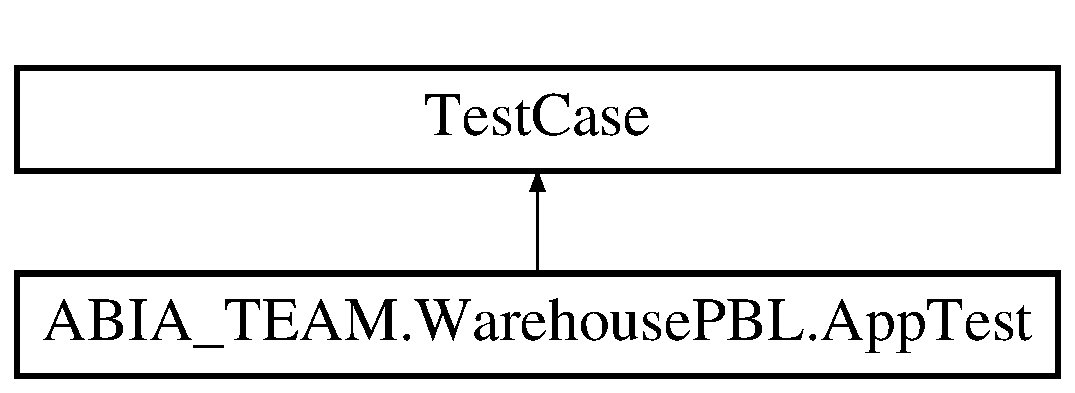
\includegraphics[height=2.000000cm]{class_a_b_i_a___t_e_a_m_1_1_warehouse_p_b_l_1_1_app_test}
\end{center}
\end{figure}
\subsection*{Public Member Functions}
\begin{DoxyCompactItemize}
\item 
\mbox{\hyperlink{class_a_b_i_a___t_e_a_m_1_1_warehouse_p_b_l_1_1_app_test_a950e4648e0c712eb08f89004c45b5097}{App\+Test}} (String test\+Name)
\item 
void \mbox{\hyperlink{class_a_b_i_a___t_e_a_m_1_1_warehouse_p_b_l_1_1_app_test_a90b5823f6dbfe81379aa8a0ee61e91d0}{test\+App}} ()
\end{DoxyCompactItemize}
\subsection*{Static Public Member Functions}
\begin{DoxyCompactItemize}
\item 
static Test \mbox{\hyperlink{class_a_b_i_a___t_e_a_m_1_1_warehouse_p_b_l_1_1_app_test_aa2b9b4e8808acbb07265881dd38df16a}{suite}} ()
\end{DoxyCompactItemize}


\subsection{Detailed Description}
Unit test for simple \mbox{\hyperlink{class_a_b_i_a___t_e_a_m_1_1_warehouse_p_b_l_1_1_app}{App}}. 

\subsection{Constructor \& Destructor Documentation}
\mbox{\Hypertarget{class_a_b_i_a___t_e_a_m_1_1_warehouse_p_b_l_1_1_app_test_a950e4648e0c712eb08f89004c45b5097}\label{class_a_b_i_a___t_e_a_m_1_1_warehouse_p_b_l_1_1_app_test_a950e4648e0c712eb08f89004c45b5097}} 
\index{A\+B\+I\+A\+\_\+\+T\+E\+A\+M\+::\+Warehouse\+P\+B\+L\+::\+App\+Test@{A\+B\+I\+A\+\_\+\+T\+E\+A\+M\+::\+Warehouse\+P\+B\+L\+::\+App\+Test}!App\+Test@{App\+Test}}
\index{App\+Test@{App\+Test}!A\+B\+I\+A\+\_\+\+T\+E\+A\+M\+::\+Warehouse\+P\+B\+L\+::\+App\+Test@{A\+B\+I\+A\+\_\+\+T\+E\+A\+M\+::\+Warehouse\+P\+B\+L\+::\+App\+Test}}
\subsubsection{\texorpdfstring{App\+Test()}{AppTest()}}
{\footnotesize\ttfamily A\+B\+I\+A\+\_\+\+T\+E\+A\+M.\+Warehouse\+P\+B\+L.\+App\+Test.\+App\+Test (\begin{DoxyParamCaption}\item[{String}]{test\+Name }\end{DoxyParamCaption})}

Create the test case


\begin{DoxyParams}{Parameters}
{\em test\+Name} & name of the test case \\
\hline
\end{DoxyParams}


\subsection{Member Function Documentation}
\mbox{\Hypertarget{class_a_b_i_a___t_e_a_m_1_1_warehouse_p_b_l_1_1_app_test_aa2b9b4e8808acbb07265881dd38df16a}\label{class_a_b_i_a___t_e_a_m_1_1_warehouse_p_b_l_1_1_app_test_aa2b9b4e8808acbb07265881dd38df16a}} 
\index{A\+B\+I\+A\+\_\+\+T\+E\+A\+M\+::\+Warehouse\+P\+B\+L\+::\+App\+Test@{A\+B\+I\+A\+\_\+\+T\+E\+A\+M\+::\+Warehouse\+P\+B\+L\+::\+App\+Test}!suite@{suite}}
\index{suite@{suite}!A\+B\+I\+A\+\_\+\+T\+E\+A\+M\+::\+Warehouse\+P\+B\+L\+::\+App\+Test@{A\+B\+I\+A\+\_\+\+T\+E\+A\+M\+::\+Warehouse\+P\+B\+L\+::\+App\+Test}}
\subsubsection{\texorpdfstring{suite()}{suite()}}
{\footnotesize\ttfamily static Test A\+B\+I\+A\+\_\+\+T\+E\+A\+M.\+Warehouse\+P\+B\+L.\+App\+Test.\+suite (\begin{DoxyParamCaption}{ }\end{DoxyParamCaption})\hspace{0.3cm}{\ttfamily [static]}}

\begin{DoxyReturn}{Returns}
the suite of tests being tested 
\end{DoxyReturn}
\mbox{\Hypertarget{class_a_b_i_a___t_e_a_m_1_1_warehouse_p_b_l_1_1_app_test_a90b5823f6dbfe81379aa8a0ee61e91d0}\label{class_a_b_i_a___t_e_a_m_1_1_warehouse_p_b_l_1_1_app_test_a90b5823f6dbfe81379aa8a0ee61e91d0}} 
\index{A\+B\+I\+A\+\_\+\+T\+E\+A\+M\+::\+Warehouse\+P\+B\+L\+::\+App\+Test@{A\+B\+I\+A\+\_\+\+T\+E\+A\+M\+::\+Warehouse\+P\+B\+L\+::\+App\+Test}!test\+App@{test\+App}}
\index{test\+App@{test\+App}!A\+B\+I\+A\+\_\+\+T\+E\+A\+M\+::\+Warehouse\+P\+B\+L\+::\+App\+Test@{A\+B\+I\+A\+\_\+\+T\+E\+A\+M\+::\+Warehouse\+P\+B\+L\+::\+App\+Test}}
\subsubsection{\texorpdfstring{test\+App()}{testApp()}}
{\footnotesize\ttfamily void A\+B\+I\+A\+\_\+\+T\+E\+A\+M.\+Warehouse\+P\+B\+L.\+App\+Test.\+test\+App (\begin{DoxyParamCaption}{ }\end{DoxyParamCaption})}

Rigourous Test \+:-\/) 

The documentation for this class was generated from the following file\+:\begin{DoxyCompactItemize}
\item 
src/test/java/\+A\+B\+I\+A\+\_\+\+T\+E\+A\+M/\+Warehouse\+P\+B\+L/App\+Test.\+java\end{DoxyCompactItemize}

\hypertarget{classmodelo_1_1_articulos}{}\section{modelo.\+Articulos Class Reference}
\label{classmodelo_1_1_articulos}\index{modelo.\+Articulos@{modelo.\+Articulos}}


Class \mbox{\hyperlink{classmodelo_1_1_articulos}{Articulos}}.  


\subsection*{Public Member Functions}
\begin{DoxyCompactItemize}
\item 
\mbox{\hyperlink{classmodelo_1_1_articulos_a520b1e25e7c87ed796ec2ac0db85475c}{Articulos}} (int id, String tipo, String nombre, String desc)
\begin{DoxyCompactList}\small\item\em Constructor. \end{DoxyCompactList}\item 
int \mbox{\hyperlink{classmodelo_1_1_articulos_a4784500f94b55f2cf7ed8670bf15a6ca}{get\+Id}} ()
\begin{DoxyCompactList}\small\item\em Method for get the value of the id variable. \end{DoxyCompactList}\item 
String \mbox{\hyperlink{classmodelo_1_1_articulos_a894f705611372b68e0bb520350626983}{get\+Tipo}} ()
\begin{DoxyCompactList}\small\item\em Method for get the value of the tipo variable. \end{DoxyCompactList}\item 
String \mbox{\hyperlink{classmodelo_1_1_articulos_a7782939b3b47698ff92e5349c6558b17}{get\+Nombre}} ()
\begin{DoxyCompactList}\small\item\em Method for get the value of the nombre variable. \end{DoxyCompactList}\item 
String \mbox{\hyperlink{classmodelo_1_1_articulos_ade935cf80e8c5e30bbbc31df6f1ea13a}{get\+Desc}} ()
\begin{DoxyCompactList}\small\item\em Method for get the value of the desc variable. \end{DoxyCompactList}\end{DoxyCompactItemize}


\subsection{Detailed Description}
Class \mbox{\hyperlink{classmodelo_1_1_articulos}{Articulos}}. 

\subsection{Constructor \& Destructor Documentation}
\mbox{\Hypertarget{classmodelo_1_1_articulos_a520b1e25e7c87ed796ec2ac0db85475c}\label{classmodelo_1_1_articulos_a520b1e25e7c87ed796ec2ac0db85475c}} 
\index{modelo\+::\+Articulos@{modelo\+::\+Articulos}!Articulos@{Articulos}}
\index{Articulos@{Articulos}!modelo\+::\+Articulos@{modelo\+::\+Articulos}}
\subsubsection{\texorpdfstring{Articulos()}{Articulos()}}
{\footnotesize\ttfamily modelo.\+Articulos.\+Articulos (\begin{DoxyParamCaption}\item[{int}]{id,  }\item[{String}]{tipo,  }\item[{String}]{nombre,  }\item[{String}]{desc }\end{DoxyParamCaption})}



Constructor. 


\begin{DoxyParams}{Parameters}
{\em id} & product ID \\
\hline
{\em tipo} & product type \\
\hline
{\em nombre} & product name \\
\hline
{\em desc} & product description \\
\hline
\end{DoxyParams}


\subsection{Member Function Documentation}
\mbox{\Hypertarget{classmodelo_1_1_articulos_ade935cf80e8c5e30bbbc31df6f1ea13a}\label{classmodelo_1_1_articulos_ade935cf80e8c5e30bbbc31df6f1ea13a}} 
\index{modelo\+::\+Articulos@{modelo\+::\+Articulos}!get\+Desc@{get\+Desc}}
\index{get\+Desc@{get\+Desc}!modelo\+::\+Articulos@{modelo\+::\+Articulos}}
\subsubsection{\texorpdfstring{get\+Desc()}{getDesc()}}
{\footnotesize\ttfamily String modelo.\+Articulos.\+get\+Desc (\begin{DoxyParamCaption}{ }\end{DoxyParamCaption})}



Method for get the value of the desc variable. 

\begin{DoxyReturn}{Returns}
String 
\end{DoxyReturn}
\mbox{\Hypertarget{classmodelo_1_1_articulos_a4784500f94b55f2cf7ed8670bf15a6ca}\label{classmodelo_1_1_articulos_a4784500f94b55f2cf7ed8670bf15a6ca}} 
\index{modelo\+::\+Articulos@{modelo\+::\+Articulos}!get\+Id@{get\+Id}}
\index{get\+Id@{get\+Id}!modelo\+::\+Articulos@{modelo\+::\+Articulos}}
\subsubsection{\texorpdfstring{get\+Id()}{getId()}}
{\footnotesize\ttfamily int modelo.\+Articulos.\+get\+Id (\begin{DoxyParamCaption}{ }\end{DoxyParamCaption})}



Method for get the value of the id variable. 

\begin{DoxyReturn}{Returns}
int 
\end{DoxyReturn}
\mbox{\Hypertarget{classmodelo_1_1_articulos_a7782939b3b47698ff92e5349c6558b17}\label{classmodelo_1_1_articulos_a7782939b3b47698ff92e5349c6558b17}} 
\index{modelo\+::\+Articulos@{modelo\+::\+Articulos}!get\+Nombre@{get\+Nombre}}
\index{get\+Nombre@{get\+Nombre}!modelo\+::\+Articulos@{modelo\+::\+Articulos}}
\subsubsection{\texorpdfstring{get\+Nombre()}{getNombre()}}
{\footnotesize\ttfamily String modelo.\+Articulos.\+get\+Nombre (\begin{DoxyParamCaption}{ }\end{DoxyParamCaption})}



Method for get the value of the nombre variable. 

\begin{DoxyReturn}{Returns}
String 
\end{DoxyReturn}
\mbox{\Hypertarget{classmodelo_1_1_articulos_a894f705611372b68e0bb520350626983}\label{classmodelo_1_1_articulos_a894f705611372b68e0bb520350626983}} 
\index{modelo\+::\+Articulos@{modelo\+::\+Articulos}!get\+Tipo@{get\+Tipo}}
\index{get\+Tipo@{get\+Tipo}!modelo\+::\+Articulos@{modelo\+::\+Articulos}}
\subsubsection{\texorpdfstring{get\+Tipo()}{getTipo()}}
{\footnotesize\ttfamily String modelo.\+Articulos.\+get\+Tipo (\begin{DoxyParamCaption}{ }\end{DoxyParamCaption})}



Method for get the value of the tipo variable. 

\begin{DoxyReturn}{Returns}
String 
\end{DoxyReturn}


The documentation for this class was generated from the following file\+:\begin{DoxyCompactItemize}
\item 
src/main/java/modelo/\mbox{\hyperlink{_articulos_8java}{Articulos.\+java}}\end{DoxyCompactItemize}

\hypertarget{classmodelo_test_1_1_articulos_test}{}\section{modelo\+Test.\+Articulos\+Test Class Reference}
\label{classmodelo_test_1_1_articulos_test}\index{modelo\+Test.\+Articulos\+Test@{modelo\+Test.\+Articulos\+Test}}


Class \mbox{\hyperlink{classmodelo_test_1_1_articulos_test}{Articulos\+Test}}.  


\subsection*{Public Member Functions}
\begin{DoxyCompactItemize}
\item 
\mbox{\Hypertarget{classmodelo_test_1_1_articulos_test_a846cb5c047bea230f8e351b2c12a0543}\label{classmodelo_test_1_1_articulos_test_a846cb5c047bea230f8e351b2c12a0543}} 
void \mbox{\hyperlink{classmodelo_test_1_1_articulos_test_a846cb5c047bea230f8e351b2c12a0543}{crear\+Articulo}} ()
\begin{DoxyCompactList}\small\item\em Method to cretate objects. \end{DoxyCompactList}\item 
\mbox{\Hypertarget{classmodelo_test_1_1_articulos_test_a805a40dbacae0f8177169aa47768c633}\label{classmodelo_test_1_1_articulos_test_a805a40dbacae0f8177169aa47768c633}} 
void \mbox{\hyperlink{classmodelo_test_1_1_articulos_test_a805a40dbacae0f8177169aa47768c633}{get\+Id\+Test}} ()
\begin{DoxyCompactList}\small\item\em method that tests the method get\+Id \end{DoxyCompactList}\item 
\mbox{\Hypertarget{classmodelo_test_1_1_articulos_test_a48c0712285ddd750fe5f45390d5ccf48}\label{classmodelo_test_1_1_articulos_test_a48c0712285ddd750fe5f45390d5ccf48}} 
void \mbox{\hyperlink{classmodelo_test_1_1_articulos_test_a48c0712285ddd750fe5f45390d5ccf48}{get\+Nombre\+Test}} ()
\begin{DoxyCompactList}\small\item\em method that tests the method get\+Nombre \end{DoxyCompactList}\item 
\mbox{\Hypertarget{classmodelo_test_1_1_articulos_test_ad0c98f454266688a9c8cfe1659c9a649}\label{classmodelo_test_1_1_articulos_test_ad0c98f454266688a9c8cfe1659c9a649}} 
void \mbox{\hyperlink{classmodelo_test_1_1_articulos_test_ad0c98f454266688a9c8cfe1659c9a649}{get\+Tipo\+Test}} ()
\begin{DoxyCompactList}\small\item\em method that tests the method get\+Tipo \end{DoxyCompactList}\item 
\mbox{\Hypertarget{classmodelo_test_1_1_articulos_test_a659341a9a39434a6dcca5c64e2ab650d}\label{classmodelo_test_1_1_articulos_test_a659341a9a39434a6dcca5c64e2ab650d}} 
void \mbox{\hyperlink{classmodelo_test_1_1_articulos_test_a659341a9a39434a6dcca5c64e2ab650d}{get\+Desc\+Test}} ()
\begin{DoxyCompactList}\small\item\em method that tests the method get\+Desc \end{DoxyCompactList}\end{DoxyCompactItemize}


\subsection{Detailed Description}
Class \mbox{\hyperlink{classmodelo_test_1_1_articulos_test}{Articulos\+Test}}. 

The documentation for this class was generated from the following file\+:\begin{DoxyCompactItemize}
\item 
src/test/java/modelo\+Test/\mbox{\hyperlink{_articulos_test_8java}{Articulos\+Test.\+java}}\end{DoxyCompactItemize}

\hypertarget{classwarehouse_p_b_l_1_1_barrier}{}\section{warehouse\+P\+B\+L.\+Barrier Class Reference}
\label{classwarehouse_p_b_l_1_1_barrier}\index{warehouse\+P\+B\+L.\+Barrier@{warehouse\+P\+B\+L.\+Barrier}}
\subsection*{Public Member Functions}
\begin{DoxyCompactItemize}
\item 
\mbox{\Hypertarget{classwarehouse_p_b_l_1_1_barrier_a4e93f9098bcec1f263be2c9cde1d9983}\label{classwarehouse_p_b_l_1_1_barrier_a4e93f9098bcec1f263be2c9cde1d9983}} 
{\bfseries Barrier} (int n\+Entry)
\end{DoxyCompactItemize}


The documentation for this class was generated from the following file\+:\begin{DoxyCompactItemize}
\item 
src/main/java/warehouse\+P\+B\+L/Barrier.\+java\end{DoxyCompactItemize}

\hypertarget{classmodelo_1_1_order}{}\section{modelo.\+Order Class Reference}
\label{classmodelo_1_1_order}\index{modelo.\+Order@{modelo.\+Order}}


Class \mbox{\hyperlink{classmodelo_1_1_order}{Order}}.  


\subsection*{Public Member Functions}
\begin{DoxyCompactItemize}
\item 
\mbox{\hyperlink{classmodelo_1_1_order_a413d8d424a685bc7c454593c55494c51}{Order}} (int id, \mbox{\hyperlink{classmodelo_1_1_posicion}{Posicion}} posicion\+Final, List$<$ \mbox{\hyperlink{classmodelo_1_1_task}{Task}} $>$ lista, String estado)
\begin{DoxyCompactList}\small\item\em Constructor. \end{DoxyCompactList}\item 
String \mbox{\hyperlink{classmodelo_1_1_order_a022a04a9662463356a74e95b723d16fc}{get\+Estado}} ()
\begin{DoxyCompactList}\small\item\em Method for get the value of the estado variable. \end{DoxyCompactList}\item 
void \mbox{\hyperlink{classmodelo_1_1_order_ae01e30a69b5efd08f428f08a75756ca6}{set\+Estado}} (String estado)
\begin{DoxyCompactList}\small\item\em Method for determine the estado of the \mbox{\hyperlink{classmodelo_1_1_order}{Order}}. \end{DoxyCompactList}\item 
int \mbox{\hyperlink{classmodelo_1_1_order_a6eed9b98ef4db951d02fe77f8f1430b1}{get\+Id}} ()
\begin{DoxyCompactList}\small\item\em Method for get the value of the id variable. \end{DoxyCompactList}\item 
\mbox{\hyperlink{classmodelo_1_1_posicion}{Posicion}} \mbox{\hyperlink{classmodelo_1_1_order_a65b8d00aa11928a30bbe069540bb182f}{get\+Posicion\+Final}} ()
\begin{DoxyCompactList}\small\item\em Method for get the value of the posicion\+Final variable. \end{DoxyCompactList}\item 
List$<$ \mbox{\hyperlink{classmodelo_1_1_task}{Task}} $>$ \mbox{\hyperlink{classmodelo_1_1_order_a63df0012d498a6d188e54bae1a355d6e}{get\+Lista\+Task}} ()
\begin{DoxyCompactList}\small\item\em Method for get the value of the lista\+Task variable. \end{DoxyCompactList}\end{DoxyCompactItemize}


\subsection{Detailed Description}
Class \mbox{\hyperlink{classmodelo_1_1_order}{Order}}. 

\subsection{Constructor \& Destructor Documentation}
\mbox{\Hypertarget{classmodelo_1_1_order_a413d8d424a685bc7c454593c55494c51}\label{classmodelo_1_1_order_a413d8d424a685bc7c454593c55494c51}} 
\index{modelo\+::\+Order@{modelo\+::\+Order}!Order@{Order}}
\index{Order@{Order}!modelo\+::\+Order@{modelo\+::\+Order}}
\subsubsection{\texorpdfstring{Order()}{Order()}}
{\footnotesize\ttfamily modelo.\+Order.\+Order (\begin{DoxyParamCaption}\item[{int}]{id,  }\item[{\mbox{\hyperlink{classmodelo_1_1_posicion}{Posicion}}}]{posicion\+Final,  }\item[{List$<$ \mbox{\hyperlink{classmodelo_1_1_task}{Task}} $>$}]{lista,  }\item[{String}]{estado }\end{DoxyParamCaption})}



Constructor. 


\begin{DoxyParams}{Parameters}
{\em id} & \mbox{\hyperlink{classmodelo_1_1_order}{Order}} ID \\
\hline
{\em posicion\+Final} & Position in which the products must be finished \\
\hline
{\em lista} & List of all tasks that the order has \\
\hline
\end{DoxyParams}


\subsection{Member Function Documentation}
\mbox{\Hypertarget{classmodelo_1_1_order_a022a04a9662463356a74e95b723d16fc}\label{classmodelo_1_1_order_a022a04a9662463356a74e95b723d16fc}} 
\index{modelo\+::\+Order@{modelo\+::\+Order}!get\+Estado@{get\+Estado}}
\index{get\+Estado@{get\+Estado}!modelo\+::\+Order@{modelo\+::\+Order}}
\subsubsection{\texorpdfstring{get\+Estado()}{getEstado()}}
{\footnotesize\ttfamily String modelo.\+Order.\+get\+Estado (\begin{DoxyParamCaption}{ }\end{DoxyParamCaption})}



Method for get the value of the estado variable. 

\begin{DoxyReturn}{Returns}
String 
\end{DoxyReturn}
\mbox{\Hypertarget{classmodelo_1_1_order_a6eed9b98ef4db951d02fe77f8f1430b1}\label{classmodelo_1_1_order_a6eed9b98ef4db951d02fe77f8f1430b1}} 
\index{modelo\+::\+Order@{modelo\+::\+Order}!get\+Id@{get\+Id}}
\index{get\+Id@{get\+Id}!modelo\+::\+Order@{modelo\+::\+Order}}
\subsubsection{\texorpdfstring{get\+Id()}{getId()}}
{\footnotesize\ttfamily int modelo.\+Order.\+get\+Id (\begin{DoxyParamCaption}{ }\end{DoxyParamCaption})}



Method for get the value of the id variable. 

\begin{DoxyReturn}{Returns}
int 
\end{DoxyReturn}
\mbox{\Hypertarget{classmodelo_1_1_order_a63df0012d498a6d188e54bae1a355d6e}\label{classmodelo_1_1_order_a63df0012d498a6d188e54bae1a355d6e}} 
\index{modelo\+::\+Order@{modelo\+::\+Order}!get\+Lista\+Task@{get\+Lista\+Task}}
\index{get\+Lista\+Task@{get\+Lista\+Task}!modelo\+::\+Order@{modelo\+::\+Order}}
\subsubsection{\texorpdfstring{get\+Lista\+Task()}{getListaTask()}}
{\footnotesize\ttfamily List$<$\mbox{\hyperlink{classmodelo_1_1_task}{Task}}$>$ modelo.\+Order.\+get\+Lista\+Task (\begin{DoxyParamCaption}{ }\end{DoxyParamCaption})}



Method for get the value of the lista\+Task variable. 

\begin{DoxyReturn}{Returns}
List$<$\+Task$>$ 
\end{DoxyReturn}
\mbox{\Hypertarget{classmodelo_1_1_order_a65b8d00aa11928a30bbe069540bb182f}\label{classmodelo_1_1_order_a65b8d00aa11928a30bbe069540bb182f}} 
\index{modelo\+::\+Order@{modelo\+::\+Order}!get\+Posicion\+Final@{get\+Posicion\+Final}}
\index{get\+Posicion\+Final@{get\+Posicion\+Final}!modelo\+::\+Order@{modelo\+::\+Order}}
\subsubsection{\texorpdfstring{get\+Posicion\+Final()}{getPosicionFinal()}}
{\footnotesize\ttfamily \mbox{\hyperlink{classmodelo_1_1_posicion}{Posicion}} modelo.\+Order.\+get\+Posicion\+Final (\begin{DoxyParamCaption}{ }\end{DoxyParamCaption})}



Method for get the value of the posicion\+Final variable. 

\begin{DoxyReturn}{Returns}
\mbox{\hyperlink{classmodelo_1_1_posicion}{Posicion}} 
\end{DoxyReturn}
\mbox{\Hypertarget{classmodelo_1_1_order_ae01e30a69b5efd08f428f08a75756ca6}\label{classmodelo_1_1_order_ae01e30a69b5efd08f428f08a75756ca6}} 
\index{modelo\+::\+Order@{modelo\+::\+Order}!set\+Estado@{set\+Estado}}
\index{set\+Estado@{set\+Estado}!modelo\+::\+Order@{modelo\+::\+Order}}
\subsubsection{\texorpdfstring{set\+Estado()}{setEstado()}}
{\footnotesize\ttfamily void modelo.\+Order.\+set\+Estado (\begin{DoxyParamCaption}\item[{String}]{estado }\end{DoxyParamCaption})}



Method for determine the estado of the \mbox{\hyperlink{classmodelo_1_1_order}{Order}}. 


\begin{DoxyParams}{Parameters}
{\em estado} & Status of the order \\
\hline
\end{DoxyParams}


The documentation for this class was generated from the following file\+:\begin{DoxyCompactItemize}
\item 
src/main/java/modelo/\mbox{\hyperlink{_order_8java}{Order.\+java}}\end{DoxyCompactItemize}

\hypertarget{classmodelo_test_1_1_order_test}{}\section{modelo\+Test.\+Order\+Test Class Reference}
\label{classmodelo_test_1_1_order_test}\index{modelo\+Test.\+Order\+Test@{modelo\+Test.\+Order\+Test}}


Class \mbox{\hyperlink{classmodelo_test_1_1_order_test}{Order\+Test}}.  


\subsection*{Public Member Functions}
\begin{DoxyCompactItemize}
\item 
\mbox{\Hypertarget{classmodelo_test_1_1_order_test_aef8b55bb4107f5ee25b4c187b2fdb069}\label{classmodelo_test_1_1_order_test_aef8b55bb4107f5ee25b4c187b2fdb069}} 
void \mbox{\hyperlink{classmodelo_test_1_1_order_test_aef8b55bb4107f5ee25b4c187b2fdb069}{crear\+Order}} ()
\begin{DoxyCompactList}\small\item\em Method to cretate objects. \end{DoxyCompactList}\item 
\mbox{\Hypertarget{classmodelo_test_1_1_order_test_a5a7f78b4f7439d54e6e5f0749fd6e61c}\label{classmodelo_test_1_1_order_test_a5a7f78b4f7439d54e6e5f0749fd6e61c}} 
void \mbox{\hyperlink{classmodelo_test_1_1_order_test_a5a7f78b4f7439d54e6e5f0749fd6e61c}{get\+Estado\+Test}} ()
\begin{DoxyCompactList}\small\item\em method that tests the method get\+Estado \end{DoxyCompactList}\item 
\mbox{\Hypertarget{classmodelo_test_1_1_order_test_a64399d59db1a5ae848057cfc758a3bf3}\label{classmodelo_test_1_1_order_test_a64399d59db1a5ae848057cfc758a3bf3}} 
void \mbox{\hyperlink{classmodelo_test_1_1_order_test_a64399d59db1a5ae848057cfc758a3bf3}{set\+Estado\+Test}} ()
\begin{DoxyCompactList}\small\item\em method that tests the method set\+Estado \end{DoxyCompactList}\item 
\mbox{\Hypertarget{classmodelo_test_1_1_order_test_a7ecc657c6d15ff0a17680bf9f694f7aa}\label{classmodelo_test_1_1_order_test_a7ecc657c6d15ff0a17680bf9f694f7aa}} 
void \mbox{\hyperlink{classmodelo_test_1_1_order_test_a7ecc657c6d15ff0a17680bf9f694f7aa}{get\+Id\+Test}} ()
\begin{DoxyCompactList}\small\item\em method that tests the method get\+Id \end{DoxyCompactList}\item 
\mbox{\Hypertarget{classmodelo_test_1_1_order_test_a7c06f3d3988acc930549e1655299d444}\label{classmodelo_test_1_1_order_test_a7c06f3d3988acc930549e1655299d444}} 
void \mbox{\hyperlink{classmodelo_test_1_1_order_test_a7c06f3d3988acc930549e1655299d444}{get\+Pos\+Final\+Test}} ()
\begin{DoxyCompactList}\small\item\em method that tests the method get\+Posicion\+Final \end{DoxyCompactList}\item 
\mbox{\Hypertarget{classmodelo_test_1_1_order_test_a1e60baf67b5be0d46cec211518d94dd5}\label{classmodelo_test_1_1_order_test_a1e60baf67b5be0d46cec211518d94dd5}} 
void \mbox{\hyperlink{classmodelo_test_1_1_order_test_a1e60baf67b5be0d46cec211518d94dd5}{get\+Lista\+Test}} ()
\begin{DoxyCompactList}\small\item\em method that tests the method get\+Posicion\+Final \end{DoxyCompactList}\end{DoxyCompactItemize}


\subsection{Detailed Description}
Class \mbox{\hyperlink{classmodelo_test_1_1_order_test}{Order\+Test}}. 

The documentation for this class was generated from the following file\+:\begin{DoxyCompactItemize}
\item 
src/test/java/modelo\+Test/\mbox{\hyperlink{_order_test_8java}{Order\+Test.\+java}}\end{DoxyCompactItemize}

\hypertarget{classmodelo_1_1_parking}{}\section{modelo.\+Parking Class Reference}
\label{classmodelo_1_1_parking}\index{modelo.\+Parking@{modelo.\+Parking}}


Class \mbox{\hyperlink{classmodelo_1_1_work_station}{Work\+Station}} extends \mbox{\hyperlink{classmodelo_1_1_posicion}{Posicion}}.  


Inheritance diagram for modelo.\+Parking\+:\begin{figure}[H]
\begin{center}
\leavevmode
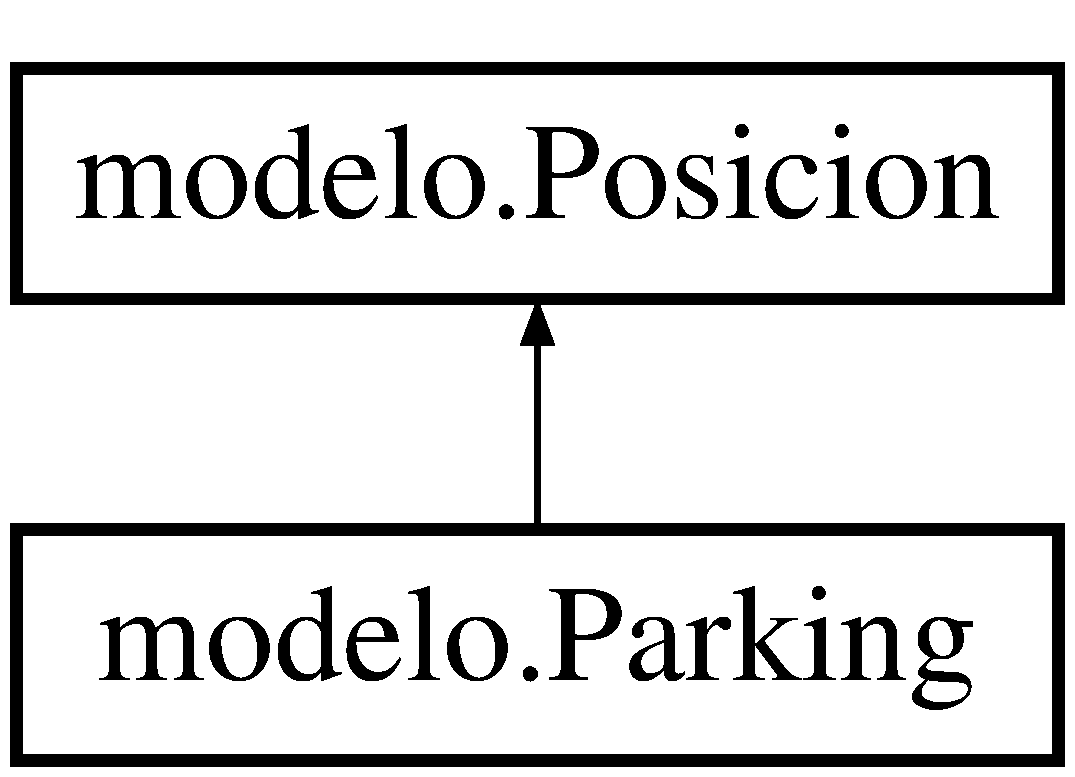
\includegraphics[height=2.000000cm]{classmodelo_1_1_parking}
\end{center}
\end{figure}
\subsection*{Public Member Functions}
\begin{DoxyCompactItemize}
\item 
\mbox{\hyperlink{classmodelo_1_1_parking_a23a70e07f89a4a9f3fab811546775ced}{Parking}} (int pos, String nombre)
\begin{DoxyCompactList}\small\item\em Constructor. \end{DoxyCompactList}\item 
void \mbox{\hyperlink{classmodelo_1_1_parking_ab2b526a6e9e8526767a0173cc3e4d406}{add\+Next\+Position}} (Posicion... pos)
\begin{DoxyCompactList}\small\item\em Method for determine which positions you can go to. \end{DoxyCompactList}\item 
\mbox{\hyperlink{classmodelo_1_1_posicion}{Posicion}} \mbox{\hyperlink{classmodelo_1_1_parking_a362f2bda656e3c9157c0589ae458c14a}{get\+Next\+Position}} ()
\begin{DoxyCompactList}\small\item\em Method for get the value of the next\+Position variable. \end{DoxyCompactList}\end{DoxyCompactItemize}


\subsection{Detailed Description}
Class \mbox{\hyperlink{classmodelo_1_1_work_station}{Work\+Station}} extends \mbox{\hyperlink{classmodelo_1_1_posicion}{Posicion}}. 

\subsection{Constructor \& Destructor Documentation}
\mbox{\Hypertarget{classmodelo_1_1_parking_a23a70e07f89a4a9f3fab811546775ced}\label{classmodelo_1_1_parking_a23a70e07f89a4a9f3fab811546775ced}} 
\index{modelo\+::\+Parking@{modelo\+::\+Parking}!Parking@{Parking}}
\index{Parking@{Parking}!modelo\+::\+Parking@{modelo\+::\+Parking}}
\subsubsection{\texorpdfstring{Parking()}{Parking()}}
{\footnotesize\ttfamily modelo.\+Parking.\+Parking (\begin{DoxyParamCaption}\item[{int}]{pos,  }\item[{String}]{nombre }\end{DoxyParamCaption})}



Constructor. 


\begin{DoxyParams}{Parameters}
{\em nombre} & position name \\
\hline
{\em pos} & Position ID or position \\
\hline
\end{DoxyParams}


\subsection{Member Function Documentation}
\mbox{\Hypertarget{classmodelo_1_1_parking_ab2b526a6e9e8526767a0173cc3e4d406}\label{classmodelo_1_1_parking_ab2b526a6e9e8526767a0173cc3e4d406}} 
\index{modelo\+::\+Parking@{modelo\+::\+Parking}!add\+Next\+Position@{add\+Next\+Position}}
\index{add\+Next\+Position@{add\+Next\+Position}!modelo\+::\+Parking@{modelo\+::\+Parking}}
\subsubsection{\texorpdfstring{add\+Next\+Position()}{addNextPosition()}}
{\footnotesize\ttfamily void modelo.\+Parking.\+add\+Next\+Position (\begin{DoxyParamCaption}\item[{Posicion...}]{pos }\end{DoxyParamCaption})}



Method for determine which positions you can go to. 


\begin{DoxyParams}{Parameters}
{\em pos} & list of next positions \\
\hline
\end{DoxyParams}
\mbox{\Hypertarget{classmodelo_1_1_parking_a362f2bda656e3c9157c0589ae458c14a}\label{classmodelo_1_1_parking_a362f2bda656e3c9157c0589ae458c14a}} 
\index{modelo\+::\+Parking@{modelo\+::\+Parking}!get\+Next\+Position@{get\+Next\+Position}}
\index{get\+Next\+Position@{get\+Next\+Position}!modelo\+::\+Parking@{modelo\+::\+Parking}}
\subsubsection{\texorpdfstring{get\+Next\+Position()}{getNextPosition()}}
{\footnotesize\ttfamily \mbox{\hyperlink{classmodelo_1_1_posicion}{Posicion}} modelo.\+Parking.\+get\+Next\+Position (\begin{DoxyParamCaption}{ }\end{DoxyParamCaption})}



Method for get the value of the next\+Position variable. 

\begin{DoxyReturn}{Returns}
\mbox{\hyperlink{classmodelo_1_1_posicion}{Posicion}} 
\end{DoxyReturn}


The documentation for this class was generated from the following file\+:\begin{DoxyCompactItemize}
\item 
src/main/java/modelo/\mbox{\hyperlink{_parking_8java}{Parking.\+java}}\end{DoxyCompactItemize}

\hypertarget{classmodelo_test_1_1_parking_test}{}\section{modelo\+Test.\+Parking\+Test Class Reference}
\label{classmodelo_test_1_1_parking_test}\index{modelo\+Test.\+Parking\+Test@{modelo\+Test.\+Parking\+Test}}


Class \mbox{\hyperlink{classmodelo_test_1_1_parking_test}{Parking\+Test}}.  


\subsection*{Public Member Functions}
\begin{DoxyCompactItemize}
\item 
\mbox{\Hypertarget{classmodelo_test_1_1_parking_test_a7ea498d3b00e02fb37ad52fc5ecb0e9f}\label{classmodelo_test_1_1_parking_test_a7ea498d3b00e02fb37ad52fc5ecb0e9f}} 
void \mbox{\hyperlink{classmodelo_test_1_1_parking_test_a7ea498d3b00e02fb37ad52fc5ecb0e9f}{crear\+Parkin}} ()
\begin{DoxyCompactList}\small\item\em Method to cretate objects. \end{DoxyCompactList}\item 
\mbox{\Hypertarget{classmodelo_test_1_1_parking_test_ae8b007838472b362cbfb6dcefbad5f15}\label{classmodelo_test_1_1_parking_test_ae8b007838472b362cbfb6dcefbad5f15}} 
void \mbox{\hyperlink{classmodelo_test_1_1_parking_test_ae8b007838472b362cbfb6dcefbad5f15}{get\+Pos\+Test}} ()
\begin{DoxyCompactList}\small\item\em method that tests the get\+Pos method \end{DoxyCompactList}\item 
\mbox{\Hypertarget{classmodelo_test_1_1_parking_test_a0e4083aeae6b528cdbe884f6d98c76a4}\label{classmodelo_test_1_1_parking_test_a0e4083aeae6b528cdbe884f6d98c76a4}} 
void \mbox{\hyperlink{classmodelo_test_1_1_parking_test_a0e4083aeae6b528cdbe884f6d98c76a4}{get\+Nombre\+Test}} ()
\begin{DoxyCompactList}\small\item\em method that tests the get\+Nombre method \end{DoxyCompactList}\item 
\mbox{\Hypertarget{classmodelo_test_1_1_parking_test_aac705e55fd569089a815b3a6f6b37e1c}\label{classmodelo_test_1_1_parking_test_aac705e55fd569089a815b3a6f6b37e1c}} 
void \mbox{\hyperlink{classmodelo_test_1_1_parking_test_aac705e55fd569089a815b3a6f6b37e1c}{Is\+Lleno\+Test}} ()
\begin{DoxyCompactList}\small\item\em method that tests the Is\+Lleno method \end{DoxyCompactList}\item 
\mbox{\Hypertarget{classmodelo_test_1_1_parking_test_a7e6beea37235da4061ccaac55bd06219}\label{classmodelo_test_1_1_parking_test_a7e6beea37235da4061ccaac55bd06219}} 
void \mbox{\hyperlink{classmodelo_test_1_1_parking_test_a7e6beea37235da4061ccaac55bd06219}{set\+Lleno\+Test}} ()
\begin{DoxyCompactList}\small\item\em method that tests the set\+Lleno method \end{DoxyCompactList}\item 
\mbox{\Hypertarget{classmodelo_test_1_1_parking_test_af691006c8fddd1c155b263c6076a43f9}\label{classmodelo_test_1_1_parking_test_af691006c8fddd1c155b263c6076a43f9}} 
void \mbox{\hyperlink{classmodelo_test_1_1_parking_test_af691006c8fddd1c155b263c6076a43f9}{add\+Next\+Position\+Test}} ()
\begin{DoxyCompactList}\small\item\em method that tests the add\+Next\+Position method \end{DoxyCompactList}\item 
\mbox{\Hypertarget{classmodelo_test_1_1_parking_test_afc3678f1497b8fb1894838ad3d305d0b}\label{classmodelo_test_1_1_parking_test_afc3678f1497b8fb1894838ad3d305d0b}} 
void \mbox{\hyperlink{classmodelo_test_1_1_parking_test_afc3678f1497b8fb1894838ad3d305d0b}{get\+Next\+Position\+Test}} ()
\begin{DoxyCompactList}\small\item\em method that tests the get\+Next\+Position method \end{DoxyCompactList}\end{DoxyCompactItemize}


\subsection{Detailed Description}
Class \mbox{\hyperlink{classmodelo_test_1_1_parking_test}{Parking\+Test}}. 

The documentation for this class was generated from the following file\+:\begin{DoxyCompactItemize}
\item 
src/test/java/modelo\+Test/\mbox{\hyperlink{_parking_test_8java}{Parking\+Test.\+java}}\end{DoxyCompactItemize}

\hypertarget{classmodelo_1_1_posicion}{}\section{modelo.\+Posicion Class Reference}
\label{classmodelo_1_1_posicion}\index{modelo.\+Posicion@{modelo.\+Posicion}}


Class \mbox{\hyperlink{classmodelo_1_1_posicion}{Posicion}}.  


Inheritance diagram for modelo.\+Posicion\+:\begin{figure}[H]
\begin{center}
\leavevmode
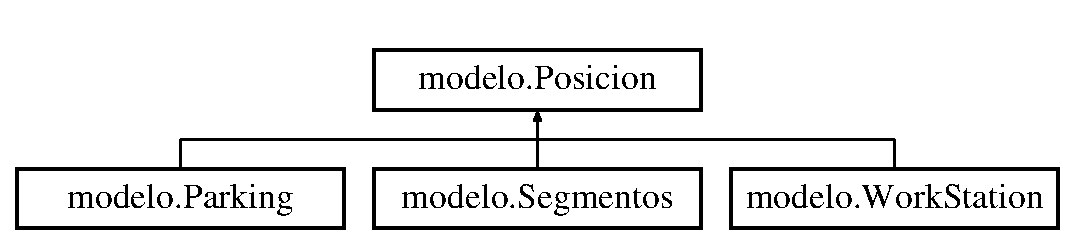
\includegraphics[height=2.000000cm]{classmodelo_1_1_posicion}
\end{center}
\end{figure}
\subsection*{Public Member Functions}
\begin{DoxyCompactItemize}
\item 
\mbox{\hyperlink{classmodelo_1_1_posicion_a8071cf7469c2dddabf012cde36d1ed78}{Posicion}} (int id, String nombre)
\begin{DoxyCompactList}\small\item\em Constructor. \end{DoxyCompactList}\item 
int \mbox{\hyperlink{classmodelo_1_1_posicion_ad81fc23f1ccae2caa6fe85ed510d8925}{get\+Id}} ()
\begin{DoxyCompactList}\small\item\em Method for get the value of the id variable. \end{DoxyCompactList}\item 
boolean \mbox{\hyperlink{classmodelo_1_1_posicion_acaad3114bb7123d7b9c75c82a50d5a4e}{is\+Lleno}} ()
\begin{DoxyCompactList}\small\item\em Method for get the value of the lleno variable. \end{DoxyCompactList}\item 
void \mbox{\hyperlink{classmodelo_1_1_posicion_a508d39b3c2031a5bbbf9bb3f6a4f3e5d}{set\+Lleno}} (boolean lleno)
\begin{DoxyCompactList}\small\item\em Method for determine the state of the position. \end{DoxyCompactList}\item 
String \mbox{\hyperlink{classmodelo_1_1_posicion_af349bd584f20e43466bdc838469f95df}{get\+Nombre}} ()
\begin{DoxyCompactList}\small\item\em Method for get the value of the nombre variable. \end{DoxyCompactList}\item 
abstract void \mbox{\hyperlink{classmodelo_1_1_posicion_a6523ec41020a97ad305b9997c88f363c}{add\+Next\+Position}} (Posicion...\+pos)
\begin{DoxyCompactList}\small\item\em Method for determine which positions you can go to. \end{DoxyCompactList}\end{DoxyCompactItemize}


\subsection{Detailed Description}
Class \mbox{\hyperlink{classmodelo_1_1_posicion}{Posicion}}. 

\subsection{Constructor \& Destructor Documentation}
\mbox{\Hypertarget{classmodelo_1_1_posicion_a8071cf7469c2dddabf012cde36d1ed78}\label{classmodelo_1_1_posicion_a8071cf7469c2dddabf012cde36d1ed78}} 
\index{modelo\+::\+Posicion@{modelo\+::\+Posicion}!Posicion@{Posicion}}
\index{Posicion@{Posicion}!modelo\+::\+Posicion@{modelo\+::\+Posicion}}
\subsubsection{\texorpdfstring{Posicion()}{Posicion()}}
{\footnotesize\ttfamily modelo.\+Posicion.\+Posicion (\begin{DoxyParamCaption}\item[{int}]{id,  }\item[{String}]{nombre }\end{DoxyParamCaption})}



Constructor. 


\begin{DoxyParams}{Parameters}
{\em nombre} & position name \\
\hline
{\em pos} & Position ID or position \\
\hline
\end{DoxyParams}


\subsection{Member Function Documentation}
\mbox{\Hypertarget{classmodelo_1_1_posicion_a6523ec41020a97ad305b9997c88f363c}\label{classmodelo_1_1_posicion_a6523ec41020a97ad305b9997c88f363c}} 
\index{modelo\+::\+Posicion@{modelo\+::\+Posicion}!add\+Next\+Position@{add\+Next\+Position}}
\index{add\+Next\+Position@{add\+Next\+Position}!modelo\+::\+Posicion@{modelo\+::\+Posicion}}
\subsubsection{\texorpdfstring{add\+Next\+Position()}{addNextPosition()}}
{\footnotesize\ttfamily abstract void modelo.\+Posicion.\+add\+Next\+Position (\begin{DoxyParamCaption}\item[{Posicion...}]{pos }\end{DoxyParamCaption})\hspace{0.3cm}{\ttfamily [abstract]}}



Method for determine which positions you can go to. 


\begin{DoxyParams}{Parameters}
{\em pos} & list of next positions \\
\hline
\end{DoxyParams}
\mbox{\Hypertarget{classmodelo_1_1_posicion_ad81fc23f1ccae2caa6fe85ed510d8925}\label{classmodelo_1_1_posicion_ad81fc23f1ccae2caa6fe85ed510d8925}} 
\index{modelo\+::\+Posicion@{modelo\+::\+Posicion}!get\+Id@{get\+Id}}
\index{get\+Id@{get\+Id}!modelo\+::\+Posicion@{modelo\+::\+Posicion}}
\subsubsection{\texorpdfstring{get\+Id()}{getId()}}
{\footnotesize\ttfamily int modelo.\+Posicion.\+get\+Id (\begin{DoxyParamCaption}{ }\end{DoxyParamCaption})}



Method for get the value of the id variable. 

\begin{DoxyReturn}{Returns}
int 
\end{DoxyReturn}
\mbox{\Hypertarget{classmodelo_1_1_posicion_af349bd584f20e43466bdc838469f95df}\label{classmodelo_1_1_posicion_af349bd584f20e43466bdc838469f95df}} 
\index{modelo\+::\+Posicion@{modelo\+::\+Posicion}!get\+Nombre@{get\+Nombre}}
\index{get\+Nombre@{get\+Nombre}!modelo\+::\+Posicion@{modelo\+::\+Posicion}}
\subsubsection{\texorpdfstring{get\+Nombre()}{getNombre()}}
{\footnotesize\ttfamily String modelo.\+Posicion.\+get\+Nombre (\begin{DoxyParamCaption}{ }\end{DoxyParamCaption})}



Method for get the value of the nombre variable. 

\begin{DoxyReturn}{Returns}
String 
\end{DoxyReturn}
\mbox{\Hypertarget{classmodelo_1_1_posicion_acaad3114bb7123d7b9c75c82a50d5a4e}\label{classmodelo_1_1_posicion_acaad3114bb7123d7b9c75c82a50d5a4e}} 
\index{modelo\+::\+Posicion@{modelo\+::\+Posicion}!is\+Lleno@{is\+Lleno}}
\index{is\+Lleno@{is\+Lleno}!modelo\+::\+Posicion@{modelo\+::\+Posicion}}
\subsubsection{\texorpdfstring{is\+Lleno()}{isLleno()}}
{\footnotesize\ttfamily boolean modelo.\+Posicion.\+is\+Lleno (\begin{DoxyParamCaption}{ }\end{DoxyParamCaption})}



Method for get the value of the lleno variable. 

\begin{DoxyReturn}{Returns}
boolean 
\end{DoxyReturn}
\mbox{\Hypertarget{classmodelo_1_1_posicion_a508d39b3c2031a5bbbf9bb3f6a4f3e5d}\label{classmodelo_1_1_posicion_a508d39b3c2031a5bbbf9bb3f6a4f3e5d}} 
\index{modelo\+::\+Posicion@{modelo\+::\+Posicion}!set\+Lleno@{set\+Lleno}}
\index{set\+Lleno@{set\+Lleno}!modelo\+::\+Posicion@{modelo\+::\+Posicion}}
\subsubsection{\texorpdfstring{set\+Lleno()}{setLleno()}}
{\footnotesize\ttfamily void modelo.\+Posicion.\+set\+Lleno (\begin{DoxyParamCaption}\item[{boolean}]{lleno }\end{DoxyParamCaption})}



Method for determine the state of the position. 


\begin{DoxyParams}{Parameters}
{\em lleno} & state of the position \\
\hline
\end{DoxyParams}


The documentation for this class was generated from the following file\+:\begin{DoxyCompactItemize}
\item 
src/main/java/modelo/\mbox{\hyperlink{_posicion_8java}{Posicion.\+java}}\end{DoxyCompactItemize}

\hypertarget{classvista_1_1_principal}{}\section{vista.\+Principal Class Reference}
\label{classvista_1_1_principal}\index{vista.\+Principal@{vista.\+Principal}}


Class \mbox{\hyperlink{classvista_1_1_principal}{Principal}}.  


\subsection*{Static Public Member Functions}
\begin{DoxyCompactItemize}
\item 
static void \mbox{\hyperlink{classvista_1_1_principal_a1b8b2d94140680bad704c39bf9ee58cb}{main}} (String\mbox{[}$\,$\mbox{]} args)
\begin{DoxyCompactList}\small\item\em main \end{DoxyCompactList}\end{DoxyCompactItemize}


\subsection{Detailed Description}
Class \mbox{\hyperlink{classvista_1_1_principal}{Principal}}. 

\subsection{Member Function Documentation}
\mbox{\Hypertarget{classvista_1_1_principal_a1b8b2d94140680bad704c39bf9ee58cb}\label{classvista_1_1_principal_a1b8b2d94140680bad704c39bf9ee58cb}} 
\index{vista\+::\+Principal@{vista\+::\+Principal}!main@{main}}
\index{main@{main}!vista\+::\+Principal@{vista\+::\+Principal}}
\subsubsection{\texorpdfstring{main()}{main()}}
{\footnotesize\ttfamily static void vista.\+Principal.\+main (\begin{DoxyParamCaption}\item[{String \mbox{[}$\,$\mbox{]}}]{args }\end{DoxyParamCaption})\hspace{0.3cm}{\ttfamily [static]}}



main 


\begin{DoxyParams}{Parameters}
{\em args} & String\mbox{[}\mbox{]} \\
\hline
\end{DoxyParams}


The documentation for this class was generated from the following file\+:\begin{DoxyCompactItemize}
\item 
src/main/java/vista/Principal.\+java\end{DoxyCompactItemize}

\hypertarget{classmodelo_1_1_recorrido}{}\section{modelo.\+Recorrido Class Reference}
\label{classmodelo_1_1_recorrido}\index{modelo.\+Recorrido@{modelo.\+Recorrido}}


Class \mbox{\hyperlink{classmodelo_1_1_recorrido}{Recorrido}}.  


\subsection*{Public Member Functions}
\begin{DoxyCompactItemize}
\item 
\mbox{\Hypertarget{classmodelo_1_1_recorrido_a6cedcfdac885aad7b83bb1b5ffdf7261}\label{classmodelo_1_1_recorrido_a6cedcfdac885aad7b83bb1b5ffdf7261}} 
\mbox{\hyperlink{classmodelo_1_1_recorrido_a6cedcfdac885aad7b83bb1b5ffdf7261}{Recorrido}} ()
\begin{DoxyCompactList}\small\item\em Constructor. \end{DoxyCompactList}\item 
void \mbox{\hyperlink{classmodelo_1_1_recorrido_a898fb136038eb311de6ff6eaba592939}{añadir\+Posicion}} (\mbox{\hyperlink{classmodelo_1_1_posicion}{Posicion}} pos)
\begin{DoxyCompactList}\small\item\em Method that adds position to the route. \end{DoxyCompactList}\item 
\mbox{\hyperlink{classmodelo_1_1_posicion}{Posicion}} \mbox{\hyperlink{classmodelo_1_1_recorrido_a30ce3f0f577225221cca2ac099a6a6b6}{get\+Siguiente}} (\mbox{\hyperlink{classmodelo_1_1_posicion}{Posicion}} pos)
\begin{DoxyCompactList}\small\item\em Method that returns you the following position of the route. \end{DoxyCompactList}\item 
\mbox{\hyperlink{classmodelo_1_1_posicion}{Posicion}} \mbox{\hyperlink{classmodelo_1_1_recorrido_ace70d961807be77d6fec75142c2e630b}{get\+Inicio}} ()
\begin{DoxyCompactList}\small\item\em Method that returns position in which the route begins. \end{DoxyCompactList}\item 
\mbox{\hyperlink{classmodelo_1_1_posicion}{Posicion}} \mbox{\hyperlink{classmodelo_1_1_recorrido_a553b3ffc252f878460d5d6ed55ea61fb}{get\+Final}} ()
\begin{DoxyCompactList}\small\item\em Method that returns position in which the route ends. \end{DoxyCompactList}\end{DoxyCompactItemize}


\subsection{Detailed Description}
Class \mbox{\hyperlink{classmodelo_1_1_recorrido}{Recorrido}}. 

\subsection{Member Function Documentation}
\mbox{\Hypertarget{classmodelo_1_1_recorrido_a898fb136038eb311de6ff6eaba592939}\label{classmodelo_1_1_recorrido_a898fb136038eb311de6ff6eaba592939}} 
\index{modelo\+::\+Recorrido@{modelo\+::\+Recorrido}!añadir\+Posicion@{añadir\+Posicion}}
\index{añadir\+Posicion@{añadir\+Posicion}!modelo\+::\+Recorrido@{modelo\+::\+Recorrido}}
\subsubsection{\texorpdfstring{añadir\+Posicion()}{añadirPosicion()}}
{\footnotesize\ttfamily void modelo.\+Recorrido.\+añadir\+Posicion (\begin{DoxyParamCaption}\item[{\mbox{\hyperlink{classmodelo_1_1_posicion}{Posicion}}}]{pos }\end{DoxyParamCaption})}



Method that adds position to the route. 


\begin{DoxyParams}{Parameters}
{\em pos} & Position to be added to the route \\
\hline
\end{DoxyParams}
\mbox{\Hypertarget{classmodelo_1_1_recorrido_a553b3ffc252f878460d5d6ed55ea61fb}\label{classmodelo_1_1_recorrido_a553b3ffc252f878460d5d6ed55ea61fb}} 
\index{modelo\+::\+Recorrido@{modelo\+::\+Recorrido}!get\+Final@{get\+Final}}
\index{get\+Final@{get\+Final}!modelo\+::\+Recorrido@{modelo\+::\+Recorrido}}
\subsubsection{\texorpdfstring{get\+Final()}{getFinal()}}
{\footnotesize\ttfamily \mbox{\hyperlink{classmodelo_1_1_posicion}{Posicion}} modelo.\+Recorrido.\+get\+Final (\begin{DoxyParamCaption}{ }\end{DoxyParamCaption})}



Method that returns position in which the route ends. 

\begin{DoxyReturn}{Returns}
\mbox{\hyperlink{classmodelo_1_1_posicion}{Posicion}} 
\end{DoxyReturn}
\mbox{\Hypertarget{classmodelo_1_1_recorrido_ace70d961807be77d6fec75142c2e630b}\label{classmodelo_1_1_recorrido_ace70d961807be77d6fec75142c2e630b}} 
\index{modelo\+::\+Recorrido@{modelo\+::\+Recorrido}!get\+Inicio@{get\+Inicio}}
\index{get\+Inicio@{get\+Inicio}!modelo\+::\+Recorrido@{modelo\+::\+Recorrido}}
\subsubsection{\texorpdfstring{get\+Inicio()}{getInicio()}}
{\footnotesize\ttfamily \mbox{\hyperlink{classmodelo_1_1_posicion}{Posicion}} modelo.\+Recorrido.\+get\+Inicio (\begin{DoxyParamCaption}{ }\end{DoxyParamCaption})}



Method that returns position in which the route begins. 

\begin{DoxyReturn}{Returns}
\mbox{\hyperlink{classmodelo_1_1_posicion}{Posicion}} 
\end{DoxyReturn}
\mbox{\Hypertarget{classmodelo_1_1_recorrido_a30ce3f0f577225221cca2ac099a6a6b6}\label{classmodelo_1_1_recorrido_a30ce3f0f577225221cca2ac099a6a6b6}} 
\index{modelo\+::\+Recorrido@{modelo\+::\+Recorrido}!get\+Siguiente@{get\+Siguiente}}
\index{get\+Siguiente@{get\+Siguiente}!modelo\+::\+Recorrido@{modelo\+::\+Recorrido}}
\subsubsection{\texorpdfstring{get\+Siguiente()}{getSiguiente()}}
{\footnotesize\ttfamily \mbox{\hyperlink{classmodelo_1_1_posicion}{Posicion}} modelo.\+Recorrido.\+get\+Siguiente (\begin{DoxyParamCaption}\item[{\mbox{\hyperlink{classmodelo_1_1_posicion}{Posicion}}}]{pos }\end{DoxyParamCaption})}



Method that returns you the following position of the route. 


\begin{DoxyParams}{Parameters}
{\em pos} & Position you are in \\
\hline
\end{DoxyParams}
\begin{DoxyReturn}{Returns}
\mbox{\hyperlink{classmodelo_1_1_posicion}{Posicion}} 
\end{DoxyReturn}


The documentation for this class was generated from the following file\+:\begin{DoxyCompactItemize}
\item 
src/main/java/modelo/Recorrido.\+java\end{DoxyCompactItemize}

\hypertarget{classmodelo_1_1_segmentos}{}\section{modelo.\+Segmentos Class Reference}
\label{classmodelo_1_1_segmentos}\index{modelo.\+Segmentos@{modelo.\+Segmentos}}


Class \mbox{\hyperlink{classmodelo_1_1_segmentos}{Segmentos}} extends \mbox{\hyperlink{classmodelo_1_1_posicion}{Posicion}}.  


Inheritance diagram for modelo.\+Segmentos\+:\begin{figure}[H]
\begin{center}
\leavevmode
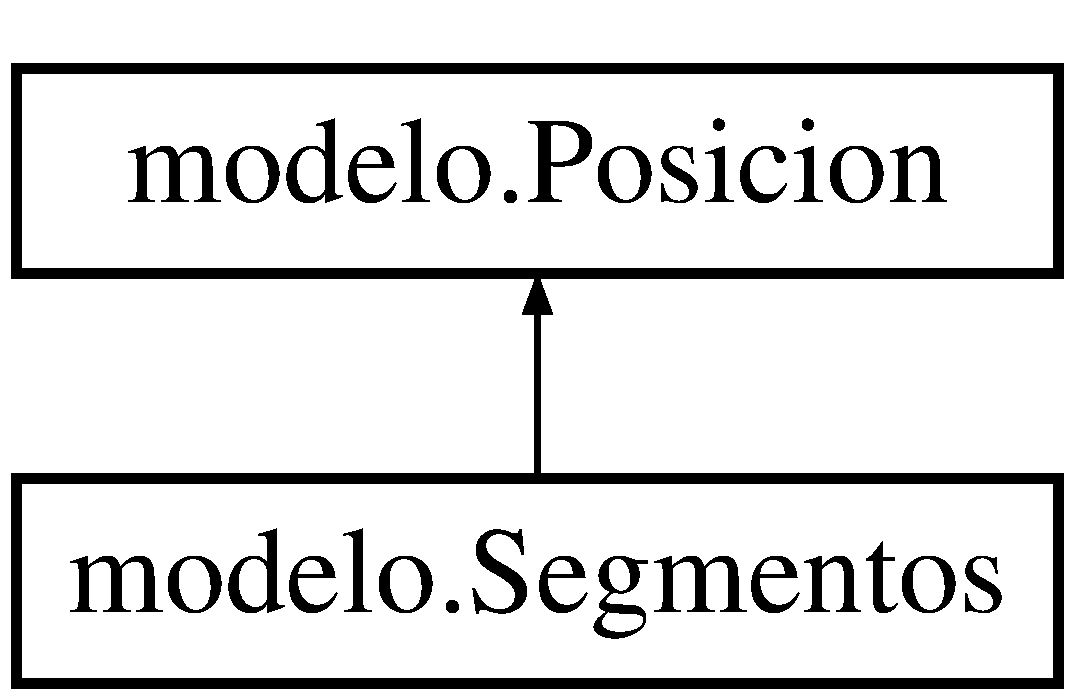
\includegraphics[height=2.000000cm]{classmodelo_1_1_segmentos}
\end{center}
\end{figure}
\subsection*{Public Member Functions}
\begin{DoxyCompactItemize}
\item 
\mbox{\hyperlink{classmodelo_1_1_segmentos_a27b81fdf669238c2851d4208ffbcb43a}{Segmentos}} (int pos, String nombre)
\begin{DoxyCompactList}\small\item\em Constructor. \end{DoxyCompactList}\item 
void \mbox{\hyperlink{classmodelo_1_1_segmentos_a287213096bb01f3a0f7b2944be99242c}{add\+Next\+Position}} (Posicion... pos)
\begin{DoxyCompactList}\small\item\em Method for determine which positions you can go to. \end{DoxyCompactList}\item 
List$<$ \mbox{\hyperlink{classmodelo_1_1_posicion}{Posicion}} $>$ \mbox{\hyperlink{classmodelo_1_1_segmentos_a33a1303cc99da1643d3bd7a897eca0cc}{get\+Next\+Position}} ()
\begin{DoxyCompactList}\small\item\em Method for get the values of the next\+Position variable. \end{DoxyCompactList}\item 
int \mbox{\hyperlink{classmodelo_1_1_segmentos_a3a0325af8cd98cdfe28294ed36012780}{get\+Distancia}} ()
\begin{DoxyCompactList}\small\item\em Method for get the values of the distancia variable. \end{DoxyCompactList}\end{DoxyCompactItemize}


\subsection{Detailed Description}
Class \mbox{\hyperlink{classmodelo_1_1_segmentos}{Segmentos}} extends \mbox{\hyperlink{classmodelo_1_1_posicion}{Posicion}}. 

\subsection{Constructor \& Destructor Documentation}
\mbox{\Hypertarget{classmodelo_1_1_segmentos_a27b81fdf669238c2851d4208ffbcb43a}\label{classmodelo_1_1_segmentos_a27b81fdf669238c2851d4208ffbcb43a}} 
\index{modelo\+::\+Segmentos@{modelo\+::\+Segmentos}!Segmentos@{Segmentos}}
\index{Segmentos@{Segmentos}!modelo\+::\+Segmentos@{modelo\+::\+Segmentos}}
\subsubsection{\texorpdfstring{Segmentos()}{Segmentos()}}
{\footnotesize\ttfamily modelo.\+Segmentos.\+Segmentos (\begin{DoxyParamCaption}\item[{int}]{pos,  }\item[{String}]{nombre }\end{DoxyParamCaption})}



Constructor. 


\begin{DoxyParams}{Parameters}
{\em nombre} & position name \\
\hline
{\em pos} & Position ID or position \\
\hline
\end{DoxyParams}


\subsection{Member Function Documentation}
\mbox{\Hypertarget{classmodelo_1_1_segmentos_a287213096bb01f3a0f7b2944be99242c}\label{classmodelo_1_1_segmentos_a287213096bb01f3a0f7b2944be99242c}} 
\index{modelo\+::\+Segmentos@{modelo\+::\+Segmentos}!add\+Next\+Position@{add\+Next\+Position}}
\index{add\+Next\+Position@{add\+Next\+Position}!modelo\+::\+Segmentos@{modelo\+::\+Segmentos}}
\subsubsection{\texorpdfstring{add\+Next\+Position()}{addNextPosition()}}
{\footnotesize\ttfamily void modelo.\+Segmentos.\+add\+Next\+Position (\begin{DoxyParamCaption}\item[{Posicion...}]{pos }\end{DoxyParamCaption})}



Method for determine which positions you can go to. 


\begin{DoxyParams}{Parameters}
{\em pos} & list of next positions \\
\hline
\end{DoxyParams}
\mbox{\Hypertarget{classmodelo_1_1_segmentos_a3a0325af8cd98cdfe28294ed36012780}\label{classmodelo_1_1_segmentos_a3a0325af8cd98cdfe28294ed36012780}} 
\index{modelo\+::\+Segmentos@{modelo\+::\+Segmentos}!get\+Distancia@{get\+Distancia}}
\index{get\+Distancia@{get\+Distancia}!modelo\+::\+Segmentos@{modelo\+::\+Segmentos}}
\subsubsection{\texorpdfstring{get\+Distancia()}{getDistancia()}}
{\footnotesize\ttfamily int modelo.\+Segmentos.\+get\+Distancia (\begin{DoxyParamCaption}{ }\end{DoxyParamCaption})}



Method for get the values of the distancia variable. 

\begin{DoxyReturn}{Returns}
int 
\end{DoxyReturn}
\mbox{\Hypertarget{classmodelo_1_1_segmentos_a33a1303cc99da1643d3bd7a897eca0cc}\label{classmodelo_1_1_segmentos_a33a1303cc99da1643d3bd7a897eca0cc}} 
\index{modelo\+::\+Segmentos@{modelo\+::\+Segmentos}!get\+Next\+Position@{get\+Next\+Position}}
\index{get\+Next\+Position@{get\+Next\+Position}!modelo\+::\+Segmentos@{modelo\+::\+Segmentos}}
\subsubsection{\texorpdfstring{get\+Next\+Position()}{getNextPosition()}}
{\footnotesize\ttfamily List$<$\mbox{\hyperlink{classmodelo_1_1_posicion}{Posicion}}$>$ modelo.\+Segmentos.\+get\+Next\+Position (\begin{DoxyParamCaption}{ }\end{DoxyParamCaption})}



Method for get the values of the next\+Position variable. 

\begin{DoxyReturn}{Returns}
Position 
\end{DoxyReturn}


The documentation for this class was generated from the following file\+:\begin{DoxyCompactItemize}
\item 
src/main/java/modelo/\mbox{\hyperlink{_segmentos_8java}{Segmentos.\+java}}\end{DoxyCompactItemize}

\hypertarget{classmodelo_test_1_1_segmentos_test}{}\section{modelo\+Test.\+Segmentos\+Test Class Reference}
\label{classmodelo_test_1_1_segmentos_test}\index{modelo\+Test.\+Segmentos\+Test@{modelo\+Test.\+Segmentos\+Test}}


Class \mbox{\hyperlink{classmodelo_test_1_1_articulos_test}{Articulos\+Test}}.  


\subsection*{Public Member Functions}
\begin{DoxyCompactItemize}
\item 
\mbox{\Hypertarget{classmodelo_test_1_1_segmentos_test_adec536c9b9233edf90250477fa4ae0fe}\label{classmodelo_test_1_1_segmentos_test_adec536c9b9233edf90250477fa4ae0fe}} 
void \mbox{\hyperlink{classmodelo_test_1_1_segmentos_test_adec536c9b9233edf90250477fa4ae0fe}{crear\+Segmentos}} ()
\begin{DoxyCompactList}\small\item\em Method to cretate objects. \end{DoxyCompactList}\item 
\mbox{\Hypertarget{classmodelo_test_1_1_segmentos_test_abc7fc571070f145ba88a5bb92eb8deb5}\label{classmodelo_test_1_1_segmentos_test_abc7fc571070f145ba88a5bb92eb8deb5}} 
void \mbox{\hyperlink{classmodelo_test_1_1_segmentos_test_abc7fc571070f145ba88a5bb92eb8deb5}{Next\+Position\+Test}} ()
\begin{DoxyCompactList}\small\item\em method that tests the Next\+Position method \end{DoxyCompactList}\item 
\mbox{\Hypertarget{classmodelo_test_1_1_segmentos_test_a038546ecb6a7d93a5356d6daa705efd8}\label{classmodelo_test_1_1_segmentos_test_a038546ecb6a7d93a5356d6daa705efd8}} 
void \mbox{\hyperlink{classmodelo_test_1_1_segmentos_test_a038546ecb6a7d93a5356d6daa705efd8}{get\+Distancia\+Test}} ()
\begin{DoxyCompactList}\small\item\em method that tests the get\+Distancia method \end{DoxyCompactList}\end{DoxyCompactItemize}


\subsection{Detailed Description}
Class \mbox{\hyperlink{classmodelo_test_1_1_articulos_test}{Articulos\+Test}}. 

The documentation for this class was generated from the following file\+:\begin{DoxyCompactItemize}
\item 
src/test/java/modelo\+Test/Segmentos\+Test.\+java\end{DoxyCompactItemize}

\hypertarget{classwarehouse_p_b_l_1_1_some_meeting_task}{}\section{warehouse\+P\+B\+L.\+Some\+Meeting\+Task Class Reference}
\label{classwarehouse_p_b_l_1_1_some_meeting_task}\index{warehouse\+P\+B\+L.\+Some\+Meeting\+Task@{warehouse\+P\+B\+L.\+Some\+Meeting\+Task}}
\subsection*{Static Public Member Functions}
\begin{DoxyCompactItemize}
\item 
\mbox{\Hypertarget{classwarehouse_p_b_l_1_1_some_meeting_task_ad32631746dce91be3960491cfbd02ee8}\label{classwarehouse_p_b_l_1_1_some_meeting_task_ad32631746dce91be3960491cfbd02ee8}} 
static void {\bfseries main} (String\mbox{[}$\,$\mbox{]} args)
\end{DoxyCompactItemize}


The documentation for this class was generated from the following file\+:\begin{DoxyCompactItemize}
\item 
src/main/java/warehouse\+P\+B\+L/Some\+Meeting\+Task.\+java\end{DoxyCompactItemize}

\hypertarget{classmodelo_1_1_task}{}\section{modelo.\+Task Class Reference}
\label{classmodelo_1_1_task}\index{modelo.\+Task@{modelo.\+Task}}


Class \mbox{\hyperlink{classmodelo_1_1_task}{Task}}.  


\subsection*{Public Member Functions}
\begin{DoxyCompactItemize}
\item 
\mbox{\hyperlink{classmodelo_1_1_task_a0c361bddb0b03c29075d7c7cd09ff625}{Task}} (int id, \mbox{\hyperlink{classmodelo_1_1_articulos}{Articulos}} articulo, String estado, \mbox{\hyperlink{classmodelo_1_1_posicion}{Posicion}} posicion\+Final)
\begin{DoxyCompactList}\small\item\em Constructor. \end{DoxyCompactList}\item 
\mbox{\hyperlink{classmodelo_1_1_posicion}{Posicion}} \mbox{\hyperlink{classmodelo_1_1_task_a98fe3bd9261ee8b560195c5256fbf4ec}{get\+Posicion\+Final}} ()
\begin{DoxyCompactList}\small\item\em Method for get the value of the posicion\+Final variable. \end{DoxyCompactList}\item 
\mbox{\hyperlink{classmodelo_1_1_vehiculo}{Vehiculo}} \mbox{\hyperlink{classmodelo_1_1_task_af3ec78e6405c7d5b912798d959b5a780}{get\+Vehiculo}} ()
\begin{DoxyCompactList}\small\item\em Method for get the value of the posicion\+Final variable. \end{DoxyCompactList}\item 
void \mbox{\hyperlink{classmodelo_1_1_task_a9303b782e49cabf729418196a2712ba0}{set\+Vehiculo}} (\mbox{\hyperlink{classmodelo_1_1_vehiculo}{Vehiculo}} vehiculo)
\begin{DoxyCompactList}\small\item\em Method for determine the vehicle of the \mbox{\hyperlink{classmodelo_1_1_task}{Task}}. \end{DoxyCompactList}\item 
Date \mbox{\hyperlink{classmodelo_1_1_task_ac1c34ccbefefc2485356474f6655fc3f}{get\+Fecha}} ()
\begin{DoxyCompactList}\small\item\em Method for get the value of the posicion\+Final variable. \end{DoxyCompactList}\item 
void \mbox{\hyperlink{classmodelo_1_1_task_af78482329f81c214c6359630ea077179}{set\+Fecha}} (Date fecha)
\begin{DoxyCompactList}\small\item\em Method for determine the date when end the \mbox{\hyperlink{classmodelo_1_1_task}{Task}}. \end{DoxyCompactList}\item 
String \mbox{\hyperlink{classmodelo_1_1_task_aaa504f1dfffb4eeba7bbe4904be070b5}{get\+Estado}} ()
\begin{DoxyCompactList}\small\item\em Method for get the value of the estado variable. \end{DoxyCompactList}\item 
void \mbox{\hyperlink{classmodelo_1_1_task_af09ff21352cab3a8d0939e6d4251d673}{set\+Estado}} (String estado)
\begin{DoxyCompactList}\small\item\em Method for determine the estado of the \mbox{\hyperlink{classmodelo_1_1_task}{Task}}. \end{DoxyCompactList}\item 
int \mbox{\hyperlink{classmodelo_1_1_task_afc746b903e969188b0ad624bb0691590}{get\+Id}} ()
\begin{DoxyCompactList}\small\item\em Method for get the value of the id variable. \end{DoxyCompactList}\item 
\mbox{\hyperlink{classmodelo_1_1_articulos}{Articulos}} \mbox{\hyperlink{classmodelo_1_1_task_a860a83d1aa53c826c49f14ab9469ed78}{get\+Articulo}} ()
\begin{DoxyCompactList}\small\item\em Method for get the value of the articulo variable. \end{DoxyCompactList}\end{DoxyCompactItemize}


\subsection{Detailed Description}
Class \mbox{\hyperlink{classmodelo_1_1_task}{Task}}. 

\subsection{Constructor \& Destructor Documentation}
\mbox{\Hypertarget{classmodelo_1_1_task_a0c361bddb0b03c29075d7c7cd09ff625}\label{classmodelo_1_1_task_a0c361bddb0b03c29075d7c7cd09ff625}} 
\index{modelo\+::\+Task@{modelo\+::\+Task}!Task@{Task}}
\index{Task@{Task}!modelo\+::\+Task@{modelo\+::\+Task}}
\subsubsection{\texorpdfstring{Task()}{Task()}}
{\footnotesize\ttfamily modelo.\+Task.\+Task (\begin{DoxyParamCaption}\item[{int}]{id,  }\item[{\mbox{\hyperlink{classmodelo_1_1_articulos}{Articulos}}}]{articulo,  }\item[{String}]{estado,  }\item[{\mbox{\hyperlink{classmodelo_1_1_posicion}{Posicion}}}]{posicion\+Final }\end{DoxyParamCaption})}



Constructor. 


\begin{DoxyParams}{Parameters}
{\em id} & \mbox{\hyperlink{classmodelo_1_1_task}{Task}} ID \\
\hline
{\em articulo} & \mbox{\hyperlink{classmodelo_1_1_task}{Task}} product \\
\hline
{\em estado} & \mbox{\hyperlink{classmodelo_1_1_task}{Task}} state \\
\hline
{\em posicion\+Final} & \mbox{\hyperlink{classmodelo_1_1_task}{Task}} final position \\
\hline
\end{DoxyParams}


\subsection{Member Function Documentation}
\mbox{\Hypertarget{classmodelo_1_1_task_a860a83d1aa53c826c49f14ab9469ed78}\label{classmodelo_1_1_task_a860a83d1aa53c826c49f14ab9469ed78}} 
\index{modelo\+::\+Task@{modelo\+::\+Task}!get\+Articulo@{get\+Articulo}}
\index{get\+Articulo@{get\+Articulo}!modelo\+::\+Task@{modelo\+::\+Task}}
\subsubsection{\texorpdfstring{get\+Articulo()}{getArticulo()}}
{\footnotesize\ttfamily \mbox{\hyperlink{classmodelo_1_1_articulos}{Articulos}} modelo.\+Task.\+get\+Articulo (\begin{DoxyParamCaption}{ }\end{DoxyParamCaption})}



Method for get the value of the articulo variable. 

\begin{DoxyReturn}{Returns}
\mbox{\hyperlink{classmodelo_1_1_articulos}{Articulos}} 
\end{DoxyReturn}
\mbox{\Hypertarget{classmodelo_1_1_task_aaa504f1dfffb4eeba7bbe4904be070b5}\label{classmodelo_1_1_task_aaa504f1dfffb4eeba7bbe4904be070b5}} 
\index{modelo\+::\+Task@{modelo\+::\+Task}!get\+Estado@{get\+Estado}}
\index{get\+Estado@{get\+Estado}!modelo\+::\+Task@{modelo\+::\+Task}}
\subsubsection{\texorpdfstring{get\+Estado()}{getEstado()}}
{\footnotesize\ttfamily String modelo.\+Task.\+get\+Estado (\begin{DoxyParamCaption}{ }\end{DoxyParamCaption})}



Method for get the value of the estado variable. 

\begin{DoxyReturn}{Returns}
String 
\end{DoxyReturn}
\mbox{\Hypertarget{classmodelo_1_1_task_ac1c34ccbefefc2485356474f6655fc3f}\label{classmodelo_1_1_task_ac1c34ccbefefc2485356474f6655fc3f}} 
\index{modelo\+::\+Task@{modelo\+::\+Task}!get\+Fecha@{get\+Fecha}}
\index{get\+Fecha@{get\+Fecha}!modelo\+::\+Task@{modelo\+::\+Task}}
\subsubsection{\texorpdfstring{get\+Fecha()}{getFecha()}}
{\footnotesize\ttfamily Date modelo.\+Task.\+get\+Fecha (\begin{DoxyParamCaption}{ }\end{DoxyParamCaption})}



Method for get the value of the posicion\+Final variable. 

\begin{DoxyReturn}{Returns}
\mbox{\hyperlink{classmodelo_1_1_posicion}{Posicion}} 
\end{DoxyReturn}
\mbox{\Hypertarget{classmodelo_1_1_task_afc746b903e969188b0ad624bb0691590}\label{classmodelo_1_1_task_afc746b903e969188b0ad624bb0691590}} 
\index{modelo\+::\+Task@{modelo\+::\+Task}!get\+Id@{get\+Id}}
\index{get\+Id@{get\+Id}!modelo\+::\+Task@{modelo\+::\+Task}}
\subsubsection{\texorpdfstring{get\+Id()}{getId()}}
{\footnotesize\ttfamily int modelo.\+Task.\+get\+Id (\begin{DoxyParamCaption}{ }\end{DoxyParamCaption})}



Method for get the value of the id variable. 

\begin{DoxyReturn}{Returns}
int 
\end{DoxyReturn}
\mbox{\Hypertarget{classmodelo_1_1_task_a98fe3bd9261ee8b560195c5256fbf4ec}\label{classmodelo_1_1_task_a98fe3bd9261ee8b560195c5256fbf4ec}} 
\index{modelo\+::\+Task@{modelo\+::\+Task}!get\+Posicion\+Final@{get\+Posicion\+Final}}
\index{get\+Posicion\+Final@{get\+Posicion\+Final}!modelo\+::\+Task@{modelo\+::\+Task}}
\subsubsection{\texorpdfstring{get\+Posicion\+Final()}{getPosicionFinal()}}
{\footnotesize\ttfamily \mbox{\hyperlink{classmodelo_1_1_posicion}{Posicion}} modelo.\+Task.\+get\+Posicion\+Final (\begin{DoxyParamCaption}{ }\end{DoxyParamCaption})}



Method for get the value of the posicion\+Final variable. 

\begin{DoxyReturn}{Returns}
\mbox{\hyperlink{classmodelo_1_1_posicion}{Posicion}} 
\end{DoxyReturn}
\mbox{\Hypertarget{classmodelo_1_1_task_af3ec78e6405c7d5b912798d959b5a780}\label{classmodelo_1_1_task_af3ec78e6405c7d5b912798d959b5a780}} 
\index{modelo\+::\+Task@{modelo\+::\+Task}!get\+Vehiculo@{get\+Vehiculo}}
\index{get\+Vehiculo@{get\+Vehiculo}!modelo\+::\+Task@{modelo\+::\+Task}}
\subsubsection{\texorpdfstring{get\+Vehiculo()}{getVehiculo()}}
{\footnotesize\ttfamily \mbox{\hyperlink{classmodelo_1_1_vehiculo}{Vehiculo}} modelo.\+Task.\+get\+Vehiculo (\begin{DoxyParamCaption}{ }\end{DoxyParamCaption})}



Method for get the value of the posicion\+Final variable. 

\begin{DoxyReturn}{Returns}
\mbox{\hyperlink{classmodelo_1_1_posicion}{Posicion}} 
\end{DoxyReturn}
\mbox{\Hypertarget{classmodelo_1_1_task_af09ff21352cab3a8d0939e6d4251d673}\label{classmodelo_1_1_task_af09ff21352cab3a8d0939e6d4251d673}} 
\index{modelo\+::\+Task@{modelo\+::\+Task}!set\+Estado@{set\+Estado}}
\index{set\+Estado@{set\+Estado}!modelo\+::\+Task@{modelo\+::\+Task}}
\subsubsection{\texorpdfstring{set\+Estado()}{setEstado()}}
{\footnotesize\ttfamily void modelo.\+Task.\+set\+Estado (\begin{DoxyParamCaption}\item[{String}]{estado }\end{DoxyParamCaption})}



Method for determine the estado of the \mbox{\hyperlink{classmodelo_1_1_task}{Task}}. 


\begin{DoxyParams}{Parameters}
{\em estado} & state of the task \\
\hline
\end{DoxyParams}
\mbox{\Hypertarget{classmodelo_1_1_task_af78482329f81c214c6359630ea077179}\label{classmodelo_1_1_task_af78482329f81c214c6359630ea077179}} 
\index{modelo\+::\+Task@{modelo\+::\+Task}!set\+Fecha@{set\+Fecha}}
\index{set\+Fecha@{set\+Fecha}!modelo\+::\+Task@{modelo\+::\+Task}}
\subsubsection{\texorpdfstring{set\+Fecha()}{setFecha()}}
{\footnotesize\ttfamily void modelo.\+Task.\+set\+Fecha (\begin{DoxyParamCaption}\item[{Date}]{fecha }\end{DoxyParamCaption})}



Method for determine the date when end the \mbox{\hyperlink{classmodelo_1_1_task}{Task}}. 


\begin{DoxyParams}{Parameters}
{\em fecha} & the date when end the work \\
\hline
\end{DoxyParams}
\mbox{\Hypertarget{classmodelo_1_1_task_a9303b782e49cabf729418196a2712ba0}\label{classmodelo_1_1_task_a9303b782e49cabf729418196a2712ba0}} 
\index{modelo\+::\+Task@{modelo\+::\+Task}!set\+Vehiculo@{set\+Vehiculo}}
\index{set\+Vehiculo@{set\+Vehiculo}!modelo\+::\+Task@{modelo\+::\+Task}}
\subsubsection{\texorpdfstring{set\+Vehiculo()}{setVehiculo()}}
{\footnotesize\ttfamily void modelo.\+Task.\+set\+Vehiculo (\begin{DoxyParamCaption}\item[{\mbox{\hyperlink{classmodelo_1_1_vehiculo}{Vehiculo}}}]{vehiculo }\end{DoxyParamCaption})}



Method for determine the vehicle of the \mbox{\hyperlink{classmodelo_1_1_task}{Task}}. 


\begin{DoxyParams}{Parameters}
{\em vehiculo} & the vehicle that will do the task \\
\hline
\end{DoxyParams}


The documentation for this class was generated from the following file\+:\begin{DoxyCompactItemize}
\item 
src/main/java/modelo/\mbox{\hyperlink{_task_8java}{Task.\+java}}\end{DoxyCompactItemize}

\hypertarget{classmodelo_test_1_1_task_test}{}\section{modelo\+Test.\+Task\+Test Class Reference}
\label{classmodelo_test_1_1_task_test}\index{modelo\+Test.\+Task\+Test@{modelo\+Test.\+Task\+Test}}


Class \mbox{\hyperlink{classmodelo_test_1_1_task_test}{Task\+Test}}.  


\subsection*{Public Member Functions}
\begin{DoxyCompactItemize}
\item 
\mbox{\Hypertarget{classmodelo_test_1_1_task_test_a3c94bd5473173fc7bfcdf8019b0eae07}\label{classmodelo_test_1_1_task_test_a3c94bd5473173fc7bfcdf8019b0eae07}} 
void \mbox{\hyperlink{classmodelo_test_1_1_task_test_a3c94bd5473173fc7bfcdf8019b0eae07}{crear\+Task}} ()
\begin{DoxyCompactList}\small\item\em Method to cretate objects. \end{DoxyCompactList}\item 
\mbox{\Hypertarget{classmodelo_test_1_1_task_test_a8af6b2ec3314c104d23c6cbad5eaee11}\label{classmodelo_test_1_1_task_test_a8af6b2ec3314c104d23c6cbad5eaee11}} 
void \mbox{\hyperlink{classmodelo_test_1_1_task_test_a8af6b2ec3314c104d23c6cbad5eaee11}{get\+Pos\+Final\+Test}} ()
\begin{DoxyCompactList}\small\item\em method that tests the method get\+Posicion\+Final \end{DoxyCompactList}\item 
\mbox{\Hypertarget{classmodelo_test_1_1_task_test_afef59d8849fd5b9b205c673d732cf6d2}\label{classmodelo_test_1_1_task_test_afef59d8849fd5b9b205c673d732cf6d2}} 
void \mbox{\hyperlink{classmodelo_test_1_1_task_test_afef59d8849fd5b9b205c673d732cf6d2}{get\+Vehiculo\+Test}} ()
\begin{DoxyCompactList}\small\item\em method that tests the method get\+Vehiculo \end{DoxyCompactList}\item 
\mbox{\Hypertarget{classmodelo_test_1_1_task_test_a3716dfd7d3e84093e271e2aeaf7f7d7e}\label{classmodelo_test_1_1_task_test_a3716dfd7d3e84093e271e2aeaf7f7d7e}} 
void \mbox{\hyperlink{classmodelo_test_1_1_task_test_a3716dfd7d3e84093e271e2aeaf7f7d7e}{set\+Vehiculo\+Test}} ()
\begin{DoxyCompactList}\small\item\em method that tests the method set\+Vehiculo \end{DoxyCompactList}\item 
\mbox{\Hypertarget{classmodelo_test_1_1_task_test_a692c5c5f5f44986790ce817907f4f8af}\label{classmodelo_test_1_1_task_test_a692c5c5f5f44986790ce817907f4f8af}} 
void \mbox{\hyperlink{classmodelo_test_1_1_task_test_a692c5c5f5f44986790ce817907f4f8af}{get\+Fecha\+Test}} ()
\begin{DoxyCompactList}\small\item\em method that tests the method get\+Fecha \end{DoxyCompactList}\item 
\mbox{\Hypertarget{classmodelo_test_1_1_task_test_aa994b8002e8a06552fc08800dd1b663c}\label{classmodelo_test_1_1_task_test_aa994b8002e8a06552fc08800dd1b663c}} 
void \mbox{\hyperlink{classmodelo_test_1_1_task_test_aa994b8002e8a06552fc08800dd1b663c}{set\+Fecha\+Test}} ()
\begin{DoxyCompactList}\small\item\em method that tests the method set\+Fecha \end{DoxyCompactList}\item 
\mbox{\Hypertarget{classmodelo_test_1_1_task_test_a93162404a604c559c8497106e7119372}\label{classmodelo_test_1_1_task_test_a93162404a604c559c8497106e7119372}} 
void \mbox{\hyperlink{classmodelo_test_1_1_task_test_a93162404a604c559c8497106e7119372}{get\+Estado\+Test}} ()
\begin{DoxyCompactList}\small\item\em method that tests the method get\+Estado \end{DoxyCompactList}\item 
\mbox{\Hypertarget{classmodelo_test_1_1_task_test_a2ada4939b7fc7dc68163856a64c8b4d7}\label{classmodelo_test_1_1_task_test_a2ada4939b7fc7dc68163856a64c8b4d7}} 
void \mbox{\hyperlink{classmodelo_test_1_1_task_test_a2ada4939b7fc7dc68163856a64c8b4d7}{set\+Estado\+Test}} ()
\begin{DoxyCompactList}\small\item\em method that tests the method set\+Estado \end{DoxyCompactList}\item 
\mbox{\Hypertarget{classmodelo_test_1_1_task_test_a794deb0d695dbd93ef788fb6c3ff16e3}\label{classmodelo_test_1_1_task_test_a794deb0d695dbd93ef788fb6c3ff16e3}} 
void \mbox{\hyperlink{classmodelo_test_1_1_task_test_a794deb0d695dbd93ef788fb6c3ff16e3}{get\+Id\+Test}} ()
\begin{DoxyCompactList}\small\item\em method that tests the method get\+Id \end{DoxyCompactList}\item 
\mbox{\Hypertarget{classmodelo_test_1_1_task_test_ac7cb90633bdd40e104b1fb9a55f4eea3}\label{classmodelo_test_1_1_task_test_ac7cb90633bdd40e104b1fb9a55f4eea3}} 
void \mbox{\hyperlink{classmodelo_test_1_1_task_test_ac7cb90633bdd40e104b1fb9a55f4eea3}{get\+Articulo\+Test}} ()
\begin{DoxyCompactList}\small\item\em method that tests the method get\+Articulo \end{DoxyCompactList}\end{DoxyCompactItemize}


\subsection{Detailed Description}
Class \mbox{\hyperlink{classmodelo_test_1_1_task_test}{Task\+Test}}. 

The documentation for this class was generated from the following file\+:\begin{DoxyCompactItemize}
\item 
src/test/java/modelo\+Test/\mbox{\hyperlink{_task_test_8java}{Task\+Test.\+java}}\end{DoxyCompactItemize}

\hypertarget{classwarehouse_p_b_l_1_1_task_thread}{}\section{warehouse\+P\+B\+L.\+Task\+Thread Class Reference}
\label{classwarehouse_p_b_l_1_1_task_thread}\index{warehouse\+P\+B\+L.\+Task\+Thread@{warehouse\+P\+B\+L.\+Task\+Thread}}
Inheritance diagram for warehouse\+P\+B\+L.\+Task\+Thread\+:\begin{figure}[H]
\begin{center}
\leavevmode
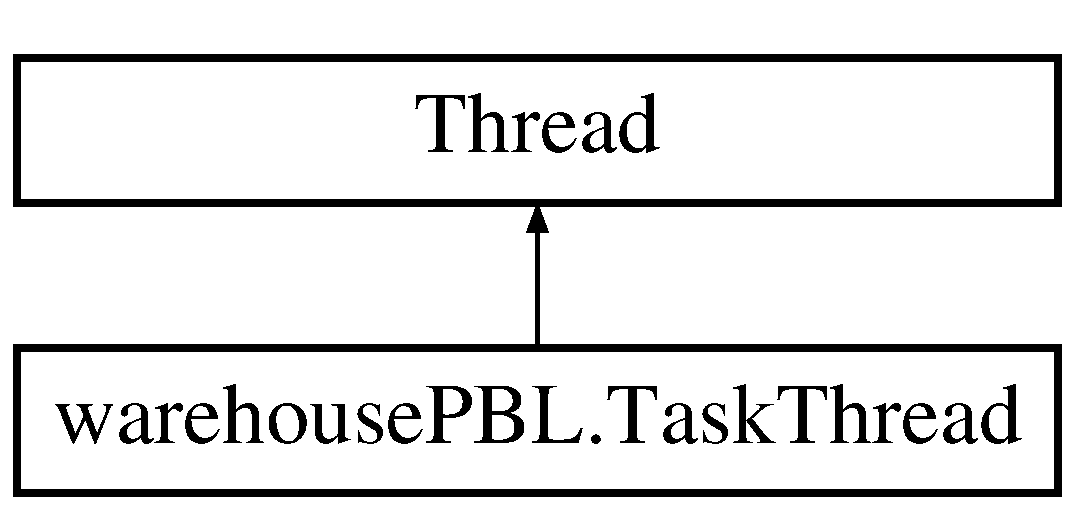
\includegraphics[height=2.000000cm]{classwarehouse_p_b_l_1_1_task_thread}
\end{center}
\end{figure}
\subsection*{Public Member Functions}
\begin{DoxyCompactItemize}
\item 
\mbox{\Hypertarget{classwarehouse_p_b_l_1_1_task_thread_a4ce9ecaa8968bd5f473804fed4f76064}\label{classwarehouse_p_b_l_1_1_task_thread_a4ce9ecaa8968bd5f473804fed4f76064}} 
{\bfseries Task\+Thread} (int id, \mbox{\hyperlink{classwarehouse_p_b_l_1_1_barrier}{Barrier}} barrier)
\item 
\mbox{\Hypertarget{classwarehouse_p_b_l_1_1_task_thread_a57b651c9ccd970a15154a3030356129b}\label{classwarehouse_p_b_l_1_1_task_thread_a57b651c9ccd970a15154a3030356129b}} 
void {\bfseries run} ()
\end{DoxyCompactItemize}


The documentation for this class was generated from the following file\+:\begin{DoxyCompactItemize}
\item 
src/main/java/warehouse\+P\+B\+L/Task\+Thread.\+java\end{DoxyCompactItemize}

\hypertarget{classmodelo_1_1_vehiculo}{}\section{modelo.\+Vehiculo Class Reference}
\label{classmodelo_1_1_vehiculo}\index{modelo.\+Vehiculo@{modelo.\+Vehiculo}}


Class \mbox{\hyperlink{classmodelo_1_1_vehiculo}{Vehiculo}}.  


\subsection*{Public Member Functions}
\begin{DoxyCompactItemize}
\item 
\mbox{\hyperlink{classmodelo_1_1_vehiculo_abff5e22c6b50ca2cefb6cb06e358e710}{Vehiculo}} (int id, String estado, \mbox{\hyperlink{classmodelo_1_1_posicion}{Posicion}} posicion)
\begin{DoxyCompactList}\small\item\em Constructor. \end{DoxyCompactList}\item 
String \mbox{\hyperlink{classmodelo_1_1_vehiculo_afc2b35fba98cc54bd67dd922db3bdc5e}{get\+Estado}} ()
\begin{DoxyCompactList}\small\item\em Method for get the value of the estado variable. \end{DoxyCompactList}\item 
void \mbox{\hyperlink{classmodelo_1_1_vehiculo_af8ba11f972f7cafec1e4f2379072c297}{set\+Estado}} (String estado)
\begin{DoxyCompactList}\small\item\em Method for determine the state of the vehicle. \end{DoxyCompactList}\item 
\mbox{\hyperlink{classmodelo_1_1_posicion}{Posicion}} \mbox{\hyperlink{classmodelo_1_1_vehiculo_a6ac6859c6824cee3ce3c8c1838fd99bd}{get\+Posicion}} ()
\begin{DoxyCompactList}\small\item\em Method for get the value of the posicion variable. \end{DoxyCompactList}\item 
int \mbox{\hyperlink{classmodelo_1_1_vehiculo_ac147041ca1529b3f926a16f67aeacbd7}{get\+Id}} ()
\begin{DoxyCompactList}\small\item\em Method for get the value of the id variable. \end{DoxyCompactList}\item 
String \mbox{\hyperlink{classmodelo_1_1_vehiculo_ac3ccc12d49158c7c20b4b9c8bb7dce85}{get\+Nombre}} ()
\begin{DoxyCompactList}\small\item\em Method for get the value of the nombre variable. \end{DoxyCompactList}\item 
void \mbox{\hyperlink{classmodelo_1_1_vehiculo_a253de2462a326996b4f427bf204ae1f9}{mover}} (\mbox{\hyperlink{classmodelo_1_1_posicion}{Posicion}} posicion)
\begin{DoxyCompactList}\small\item\em Method move vehicle to next position. \end{DoxyCompactList}\end{DoxyCompactItemize}


\subsection{Detailed Description}
Class \mbox{\hyperlink{classmodelo_1_1_vehiculo}{Vehiculo}}. 

\subsection{Constructor \& Destructor Documentation}
\mbox{\Hypertarget{classmodelo_1_1_vehiculo_abff5e22c6b50ca2cefb6cb06e358e710}\label{classmodelo_1_1_vehiculo_abff5e22c6b50ca2cefb6cb06e358e710}} 
\index{modelo\+::\+Vehiculo@{modelo\+::\+Vehiculo}!Vehiculo@{Vehiculo}}
\index{Vehiculo@{Vehiculo}!modelo\+::\+Vehiculo@{modelo\+::\+Vehiculo}}
\subsubsection{\texorpdfstring{Vehiculo()}{Vehiculo()}}
{\footnotesize\ttfamily modelo.\+Vehiculo.\+Vehiculo (\begin{DoxyParamCaption}\item[{int}]{id,  }\item[{String}]{estado,  }\item[{\mbox{\hyperlink{classmodelo_1_1_posicion}{Posicion}}}]{posicion }\end{DoxyParamCaption})}



Constructor. 


\begin{DoxyParams}{Parameters}
{\em id} & vehicle ID \\
\hline
{\em estado} & vehicle state \\
\hline
{\em posicion} & vehicle position \\
\hline
\end{DoxyParams}


\subsection{Member Function Documentation}
\mbox{\Hypertarget{classmodelo_1_1_vehiculo_afc2b35fba98cc54bd67dd922db3bdc5e}\label{classmodelo_1_1_vehiculo_afc2b35fba98cc54bd67dd922db3bdc5e}} 
\index{modelo\+::\+Vehiculo@{modelo\+::\+Vehiculo}!get\+Estado@{get\+Estado}}
\index{get\+Estado@{get\+Estado}!modelo\+::\+Vehiculo@{modelo\+::\+Vehiculo}}
\subsubsection{\texorpdfstring{get\+Estado()}{getEstado()}}
{\footnotesize\ttfamily String modelo.\+Vehiculo.\+get\+Estado (\begin{DoxyParamCaption}{ }\end{DoxyParamCaption})}



Method for get the value of the estado variable. 

\begin{DoxyReturn}{Returns}
String 
\end{DoxyReturn}
\mbox{\Hypertarget{classmodelo_1_1_vehiculo_ac147041ca1529b3f926a16f67aeacbd7}\label{classmodelo_1_1_vehiculo_ac147041ca1529b3f926a16f67aeacbd7}} 
\index{modelo\+::\+Vehiculo@{modelo\+::\+Vehiculo}!get\+Id@{get\+Id}}
\index{get\+Id@{get\+Id}!modelo\+::\+Vehiculo@{modelo\+::\+Vehiculo}}
\subsubsection{\texorpdfstring{get\+Id()}{getId()}}
{\footnotesize\ttfamily int modelo.\+Vehiculo.\+get\+Id (\begin{DoxyParamCaption}{ }\end{DoxyParamCaption})}



Method for get the value of the id variable. 

\begin{DoxyReturn}{Returns}
int 
\end{DoxyReturn}
\mbox{\Hypertarget{classmodelo_1_1_vehiculo_ac3ccc12d49158c7c20b4b9c8bb7dce85}\label{classmodelo_1_1_vehiculo_ac3ccc12d49158c7c20b4b9c8bb7dce85}} 
\index{modelo\+::\+Vehiculo@{modelo\+::\+Vehiculo}!get\+Nombre@{get\+Nombre}}
\index{get\+Nombre@{get\+Nombre}!modelo\+::\+Vehiculo@{modelo\+::\+Vehiculo}}
\subsubsection{\texorpdfstring{get\+Nombre()}{getNombre()}}
{\footnotesize\ttfamily String modelo.\+Vehiculo.\+get\+Nombre (\begin{DoxyParamCaption}{ }\end{DoxyParamCaption})}



Method for get the value of the nombre variable. 

\begin{DoxyReturn}{Returns}
String 
\end{DoxyReturn}
\mbox{\Hypertarget{classmodelo_1_1_vehiculo_a6ac6859c6824cee3ce3c8c1838fd99bd}\label{classmodelo_1_1_vehiculo_a6ac6859c6824cee3ce3c8c1838fd99bd}} 
\index{modelo\+::\+Vehiculo@{modelo\+::\+Vehiculo}!get\+Posicion@{get\+Posicion}}
\index{get\+Posicion@{get\+Posicion}!modelo\+::\+Vehiculo@{modelo\+::\+Vehiculo}}
\subsubsection{\texorpdfstring{get\+Posicion()}{getPosicion()}}
{\footnotesize\ttfamily \mbox{\hyperlink{classmodelo_1_1_posicion}{Posicion}} modelo.\+Vehiculo.\+get\+Posicion (\begin{DoxyParamCaption}{ }\end{DoxyParamCaption})}



Method for get the value of the posicion variable. 

\begin{DoxyReturn}{Returns}
\mbox{\hyperlink{classmodelo_1_1_posicion}{Posicion}} 
\end{DoxyReturn}
\mbox{\Hypertarget{classmodelo_1_1_vehiculo_a253de2462a326996b4f427bf204ae1f9}\label{classmodelo_1_1_vehiculo_a253de2462a326996b4f427bf204ae1f9}} 
\index{modelo\+::\+Vehiculo@{modelo\+::\+Vehiculo}!mover@{mover}}
\index{mover@{mover}!modelo\+::\+Vehiculo@{modelo\+::\+Vehiculo}}
\subsubsection{\texorpdfstring{mover()}{mover()}}
{\footnotesize\ttfamily void modelo.\+Vehiculo.\+mover (\begin{DoxyParamCaption}\item[{\mbox{\hyperlink{classmodelo_1_1_posicion}{Posicion}}}]{posicion }\end{DoxyParamCaption})}



Method move vehicle to next position. 


\begin{DoxyParams}{Parameters}
{\em posicion} & position of the vehicle \\
\hline
\end{DoxyParams}
\mbox{\Hypertarget{classmodelo_1_1_vehiculo_af8ba11f972f7cafec1e4f2379072c297}\label{classmodelo_1_1_vehiculo_af8ba11f972f7cafec1e4f2379072c297}} 
\index{modelo\+::\+Vehiculo@{modelo\+::\+Vehiculo}!set\+Estado@{set\+Estado}}
\index{set\+Estado@{set\+Estado}!modelo\+::\+Vehiculo@{modelo\+::\+Vehiculo}}
\subsubsection{\texorpdfstring{set\+Estado()}{setEstado()}}
{\footnotesize\ttfamily void modelo.\+Vehiculo.\+set\+Estado (\begin{DoxyParamCaption}\item[{String}]{estado }\end{DoxyParamCaption})}



Method for determine the state of the vehicle. 


\begin{DoxyParams}{Parameters}
{\em estado} & state of the vehicle \\
\hline
\end{DoxyParams}


The documentation for this class was generated from the following file\+:\begin{DoxyCompactItemize}
\item 
src/main/java/modelo/\mbox{\hyperlink{_vehiculo_8java}{Vehiculo.\+java}}\end{DoxyCompactItemize}

\hypertarget{classmodelo_test_1_1_vehiculo_test}{}\section{modelo\+Test.\+Vehiculo\+Test Class Reference}
\label{classmodelo_test_1_1_vehiculo_test}\index{modelo\+Test.\+Vehiculo\+Test@{modelo\+Test.\+Vehiculo\+Test}}


Class \mbox{\hyperlink{classmodelo_test_1_1_vehiculo_test}{Vehiculo\+Test}}.  


\subsection*{Public Member Functions}
\begin{DoxyCompactItemize}
\item 
\mbox{\Hypertarget{classmodelo_test_1_1_vehiculo_test_a698cc1dae515c04ec88bad63a195354e}\label{classmodelo_test_1_1_vehiculo_test_a698cc1dae515c04ec88bad63a195354e}} 
void \mbox{\hyperlink{classmodelo_test_1_1_vehiculo_test_a698cc1dae515c04ec88bad63a195354e}{crear\+Vehiculo}} ()
\begin{DoxyCompactList}\small\item\em Method to cretate objects. \end{DoxyCompactList}\item 
\mbox{\Hypertarget{classmodelo_test_1_1_vehiculo_test_a34b5a2b03801fa7b028232cd6617ee40}\label{classmodelo_test_1_1_vehiculo_test_a34b5a2b03801fa7b028232cd6617ee40}} 
void \mbox{\hyperlink{classmodelo_test_1_1_vehiculo_test_a34b5a2b03801fa7b028232cd6617ee40}{get\+Estado\+Test}} ()
\begin{DoxyCompactList}\small\item\em method that tests the method get\+Estado \end{DoxyCompactList}\item 
\mbox{\Hypertarget{classmodelo_test_1_1_vehiculo_test_abd28845734d433a1e84055e766d8e447}\label{classmodelo_test_1_1_vehiculo_test_abd28845734d433a1e84055e766d8e447}} 
void \mbox{\hyperlink{classmodelo_test_1_1_vehiculo_test_abd28845734d433a1e84055e766d8e447}{set\+Estado\+Test}} ()
\begin{DoxyCompactList}\small\item\em method that tests the method set\+Estado \end{DoxyCompactList}\item 
\mbox{\Hypertarget{classmodelo_test_1_1_vehiculo_test_a91fdc067b1a488b2c9daa231ac13c8a5}\label{classmodelo_test_1_1_vehiculo_test_a91fdc067b1a488b2c9daa231ac13c8a5}} 
void \mbox{\hyperlink{classmodelo_test_1_1_vehiculo_test_a91fdc067b1a488b2c9daa231ac13c8a5}{get\+Posicion\+Test}} ()
\begin{DoxyCompactList}\small\item\em method that tests the method get\+Posicion \end{DoxyCompactList}\item 
\mbox{\Hypertarget{classmodelo_test_1_1_vehiculo_test_a1388b013a8e907236a40d2232ed01388}\label{classmodelo_test_1_1_vehiculo_test_a1388b013a8e907236a40d2232ed01388}} 
void \mbox{\hyperlink{classmodelo_test_1_1_vehiculo_test_a1388b013a8e907236a40d2232ed01388}{get\+Id\+Test}} ()
\begin{DoxyCompactList}\small\item\em method that tests the method get\+Id \end{DoxyCompactList}\item 
\mbox{\Hypertarget{classmodelo_test_1_1_vehiculo_test_ab1733df7093a28b7049e79929112bc65}\label{classmodelo_test_1_1_vehiculo_test_ab1733df7093a28b7049e79929112bc65}} 
void \mbox{\hyperlink{classmodelo_test_1_1_vehiculo_test_ab1733df7093a28b7049e79929112bc65}{get\+Nombre\+Test}} ()
\begin{DoxyCompactList}\small\item\em method that tests the method get\+Nombre \end{DoxyCompactList}\item 
\mbox{\Hypertarget{classmodelo_test_1_1_vehiculo_test_a6cda67e5362be0afab0f8c793dd7d862}\label{classmodelo_test_1_1_vehiculo_test_a6cda67e5362be0afab0f8c793dd7d862}} 
void \mbox{\hyperlink{classmodelo_test_1_1_vehiculo_test_a6cda67e5362be0afab0f8c793dd7d862}{mover\+Test}} ()
\begin{DoxyCompactList}\small\item\em method that tests the method mover \end{DoxyCompactList}\end{DoxyCompactItemize}


\subsection{Detailed Description}
Class \mbox{\hyperlink{classmodelo_test_1_1_vehiculo_test}{Vehiculo\+Test}}. 

The documentation for this class was generated from the following file\+:\begin{DoxyCompactItemize}
\item 
src/test/java/modelo\+Test/\mbox{\hyperlink{_vehiculo_test_8java}{Vehiculo\+Test.\+java}}\end{DoxyCompactItemize}

\hypertarget{classmodelo_1_1_work_station}{}\section{modelo.\+Work\+Station Class Reference}
\label{classmodelo_1_1_work_station}\index{modelo.\+Work\+Station@{modelo.\+Work\+Station}}


Class \mbox{\hyperlink{classmodelo_1_1_work_station}{Work\+Station}} extends \mbox{\hyperlink{classmodelo_1_1_posicion}{Posicion}}.  


Inheritance diagram for modelo.\+Work\+Station\+:\begin{figure}[H]
\begin{center}
\leavevmode
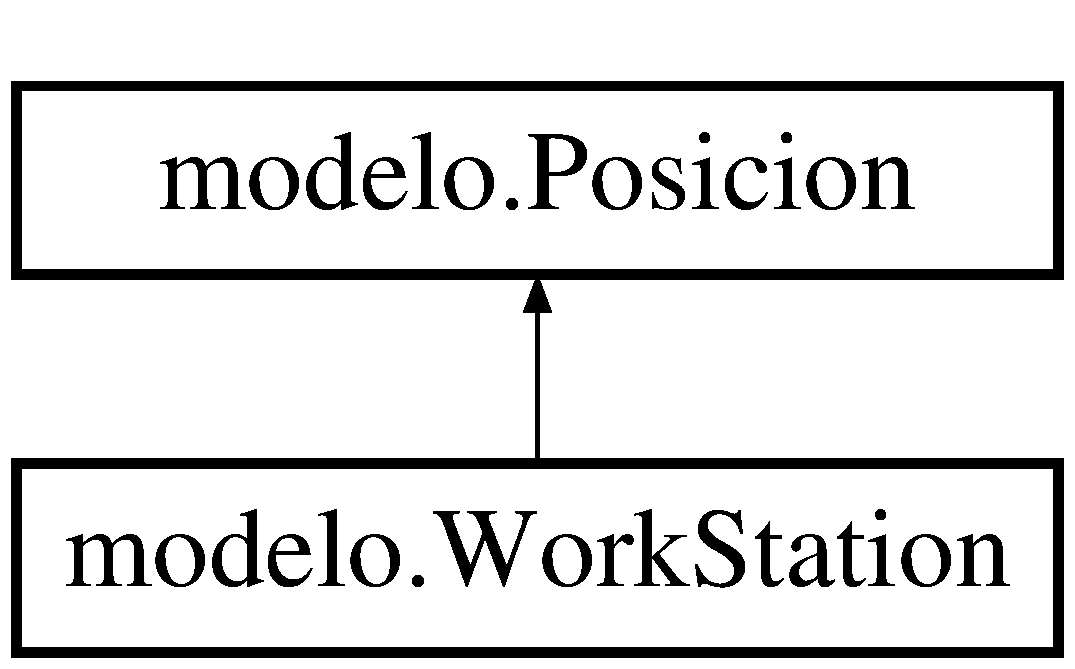
\includegraphics[height=2.000000cm]{classmodelo_1_1_work_station}
\end{center}
\end{figure}
\subsection*{Public Member Functions}
\begin{DoxyCompactItemize}
\item 
\mbox{\hyperlink{classmodelo_1_1_work_station_a04df345e4feea6715d7aafda01ed54cc}{Work\+Station}} (int pos, String nombre)
\begin{DoxyCompactList}\small\item\em Constructor. \end{DoxyCompactList}\item 
void \mbox{\hyperlink{classmodelo_1_1_work_station_ab1d63cc56798b17b893f8bb70c1445ff}{add\+Next\+Position}} (Posicion... pos)
\begin{DoxyCompactList}\small\item\em Method for determine which positions you can go to. \end{DoxyCompactList}\item 
\mbox{\hyperlink{classmodelo_1_1_posicion}{Posicion}} \mbox{\hyperlink{classmodelo_1_1_work_station_a1a51d9eb9af6508169f216cbcfb3c605}{get\+Next\+Position}} ()
\begin{DoxyCompactList}\small\item\em Method for get the value of the next\+Position variable. \end{DoxyCompactList}\item 
void \mbox{\hyperlink{classmodelo_1_1_work_station_a1d36e29aba2a6d03a918eb87d724c839}{add\+Articulo}} (\mbox{\hyperlink{classmodelo_1_1_articulos}{Articulos}} a)
\begin{DoxyCompactList}\small\item\em Method for add an \mbox{\hyperlink{classmodelo_1_1_articulos}{Articulos}} to the list\+Productos. \end{DoxyCompactList}\item 
void \mbox{\hyperlink{classmodelo_1_1_work_station_a32b6c88273b4642b6137f9b9f637650e}{delete\+Articulo}} (int index)
\begin{DoxyCompactList}\small\item\em Method for delete an product to the list\+Productos. \end{DoxyCompactList}\item 
void \mbox{\hyperlink{classmodelo_1_1_work_station_a2dad4fede50b2fc15db08f5914990d74}{delete\+Articulo}} (\mbox{\hyperlink{classmodelo_1_1_articulos}{Articulos}} a)
\begin{DoxyCompactList}\small\item\em Method for delete an product to the list\+Productos. \end{DoxyCompactList}\item 
List$<$ \mbox{\hyperlink{classmodelo_1_1_articulos}{Articulos}} $>$ \mbox{\hyperlink{classmodelo_1_1_work_station_a6b1f1a4392c9e5e31bf6168b0cc33200}{get\+List\+Productos}} ()
\begin{DoxyCompactList}\small\item\em Method for get the List of the list\+Productos. \end{DoxyCompactList}\end{DoxyCompactItemize}


\subsection{Detailed Description}
Class \mbox{\hyperlink{classmodelo_1_1_work_station}{Work\+Station}} extends \mbox{\hyperlink{classmodelo_1_1_posicion}{Posicion}}. 

\subsection{Constructor \& Destructor Documentation}
\mbox{\Hypertarget{classmodelo_1_1_work_station_a04df345e4feea6715d7aafda01ed54cc}\label{classmodelo_1_1_work_station_a04df345e4feea6715d7aafda01ed54cc}} 
\index{modelo\+::\+Work\+Station@{modelo\+::\+Work\+Station}!Work\+Station@{Work\+Station}}
\index{Work\+Station@{Work\+Station}!modelo\+::\+Work\+Station@{modelo\+::\+Work\+Station}}
\subsubsection{\texorpdfstring{Work\+Station()}{WorkStation()}}
{\footnotesize\ttfamily modelo.\+Work\+Station.\+Work\+Station (\begin{DoxyParamCaption}\item[{int}]{pos,  }\item[{String}]{nombre }\end{DoxyParamCaption})}



Constructor. 


\begin{DoxyParams}{Parameters}
{\em nombre} & position name \\
\hline
{\em pos} & Position ID or position \\
\hline
\end{DoxyParams}


\subsection{Member Function Documentation}
\mbox{\Hypertarget{classmodelo_1_1_work_station_a1d36e29aba2a6d03a918eb87d724c839}\label{classmodelo_1_1_work_station_a1d36e29aba2a6d03a918eb87d724c839}} 
\index{modelo\+::\+Work\+Station@{modelo\+::\+Work\+Station}!add\+Articulo@{add\+Articulo}}
\index{add\+Articulo@{add\+Articulo}!modelo\+::\+Work\+Station@{modelo\+::\+Work\+Station}}
\subsubsection{\texorpdfstring{add\+Articulo()}{addArticulo()}}
{\footnotesize\ttfamily void modelo.\+Work\+Station.\+add\+Articulo (\begin{DoxyParamCaption}\item[{\mbox{\hyperlink{classmodelo_1_1_articulos}{Articulos}}}]{a }\end{DoxyParamCaption})}



Method for add an \mbox{\hyperlink{classmodelo_1_1_articulos}{Articulos}} to the list\+Productos. 


\begin{DoxyParams}{Parameters}
{\em new} & Article \\
\hline
\end{DoxyParams}
\mbox{\Hypertarget{classmodelo_1_1_work_station_ab1d63cc56798b17b893f8bb70c1445ff}\label{classmodelo_1_1_work_station_ab1d63cc56798b17b893f8bb70c1445ff}} 
\index{modelo\+::\+Work\+Station@{modelo\+::\+Work\+Station}!add\+Next\+Position@{add\+Next\+Position}}
\index{add\+Next\+Position@{add\+Next\+Position}!modelo\+::\+Work\+Station@{modelo\+::\+Work\+Station}}
\subsubsection{\texorpdfstring{add\+Next\+Position()}{addNextPosition()}}
{\footnotesize\ttfamily void modelo.\+Work\+Station.\+add\+Next\+Position (\begin{DoxyParamCaption}\item[{Posicion...}]{pos }\end{DoxyParamCaption})}



Method for determine which positions you can go to. 


\begin{DoxyParams}{Parameters}
{\em pos} & list of next positions \\
\hline
\end{DoxyParams}
\mbox{\Hypertarget{classmodelo_1_1_work_station_a32b6c88273b4642b6137f9b9f637650e}\label{classmodelo_1_1_work_station_a32b6c88273b4642b6137f9b9f637650e}} 
\index{modelo\+::\+Work\+Station@{modelo\+::\+Work\+Station}!delete\+Articulo@{delete\+Articulo}}
\index{delete\+Articulo@{delete\+Articulo}!modelo\+::\+Work\+Station@{modelo\+::\+Work\+Station}}
\subsubsection{\texorpdfstring{delete\+Articulo()}{deleteArticulo()}\hspace{0.1cm}{\footnotesize\ttfamily [1/2]}}
{\footnotesize\ttfamily void modelo.\+Work\+Station.\+delete\+Articulo (\begin{DoxyParamCaption}\item[{int}]{index }\end{DoxyParamCaption})}



Method for delete an product to the list\+Productos. 


\begin{DoxyParams}{Parameters}
{\em delete} & product index \\
\hline
\end{DoxyParams}
\mbox{\Hypertarget{classmodelo_1_1_work_station_a2dad4fede50b2fc15db08f5914990d74}\label{classmodelo_1_1_work_station_a2dad4fede50b2fc15db08f5914990d74}} 
\index{modelo\+::\+Work\+Station@{modelo\+::\+Work\+Station}!delete\+Articulo@{delete\+Articulo}}
\index{delete\+Articulo@{delete\+Articulo}!modelo\+::\+Work\+Station@{modelo\+::\+Work\+Station}}
\subsubsection{\texorpdfstring{delete\+Articulo()}{deleteArticulo()}\hspace{0.1cm}{\footnotesize\ttfamily [2/2]}}
{\footnotesize\ttfamily void modelo.\+Work\+Station.\+delete\+Articulo (\begin{DoxyParamCaption}\item[{\mbox{\hyperlink{classmodelo_1_1_articulos}{Articulos}}}]{a }\end{DoxyParamCaption})}



Method for delete an product to the list\+Productos. 


\begin{DoxyParams}{Parameters}
{\em delete} & product \\
\hline
\end{DoxyParams}
\mbox{\Hypertarget{classmodelo_1_1_work_station_a6b1f1a4392c9e5e31bf6168b0cc33200}\label{classmodelo_1_1_work_station_a6b1f1a4392c9e5e31bf6168b0cc33200}} 
\index{modelo\+::\+Work\+Station@{modelo\+::\+Work\+Station}!get\+List\+Productos@{get\+List\+Productos}}
\index{get\+List\+Productos@{get\+List\+Productos}!modelo\+::\+Work\+Station@{modelo\+::\+Work\+Station}}
\subsubsection{\texorpdfstring{get\+List\+Productos()}{getListProductos()}}
{\footnotesize\ttfamily List$<$\mbox{\hyperlink{classmodelo_1_1_articulos}{Articulos}}$>$ modelo.\+Work\+Station.\+get\+List\+Productos (\begin{DoxyParamCaption}{ }\end{DoxyParamCaption})}



Method for get the List of the list\+Productos. 

\begin{DoxyReturn}{Returns}
List$<$\+Articulos$>$ 
\end{DoxyReturn}
\mbox{\Hypertarget{classmodelo_1_1_work_station_a1a51d9eb9af6508169f216cbcfb3c605}\label{classmodelo_1_1_work_station_a1a51d9eb9af6508169f216cbcfb3c605}} 
\index{modelo\+::\+Work\+Station@{modelo\+::\+Work\+Station}!get\+Next\+Position@{get\+Next\+Position}}
\index{get\+Next\+Position@{get\+Next\+Position}!modelo\+::\+Work\+Station@{modelo\+::\+Work\+Station}}
\subsubsection{\texorpdfstring{get\+Next\+Position()}{getNextPosition()}}
{\footnotesize\ttfamily \mbox{\hyperlink{classmodelo_1_1_posicion}{Posicion}} modelo.\+Work\+Station.\+get\+Next\+Position (\begin{DoxyParamCaption}{ }\end{DoxyParamCaption})}



Method for get the value of the next\+Position variable. 

\begin{DoxyReturn}{Returns}
Position 
\end{DoxyReturn}


The documentation for this class was generated from the following file\+:\begin{DoxyCompactItemize}
\item 
src/main/java/modelo/\mbox{\hyperlink{_work_station_8java}{Work\+Station.\+java}}\end{DoxyCompactItemize}

\hypertarget{classmodelo_test_1_1_work_station_test}{}\section{modelo\+Test.\+Work\+Station\+Test Class Reference}
\label{classmodelo_test_1_1_work_station_test}\index{modelo\+Test.\+Work\+Station\+Test@{modelo\+Test.\+Work\+Station\+Test}}


Class \mbox{\hyperlink{classmodelo_test_1_1_work_station_test}{Work\+Station\+Test}}.  


\subsection*{Public Member Functions}
\begin{DoxyCompactItemize}
\item 
\mbox{\Hypertarget{classmodelo_test_1_1_work_station_test_aecfdd5044fa61ddf699bd4c69a34f1c4}\label{classmodelo_test_1_1_work_station_test_aecfdd5044fa61ddf699bd4c69a34f1c4}} 
void \mbox{\hyperlink{classmodelo_test_1_1_work_station_test_aecfdd5044fa61ddf699bd4c69a34f1c4}{crear\+Vehiculo}} ()
\begin{DoxyCompactList}\small\item\em Method to cretate objects. \end{DoxyCompactList}\item 
\mbox{\Hypertarget{classmodelo_test_1_1_work_station_test_a83492675ceba62ebf1d0b93f6d931710}\label{classmodelo_test_1_1_work_station_test_a83492675ceba62ebf1d0b93f6d931710}} 
void \mbox{\hyperlink{classmodelo_test_1_1_work_station_test_a83492675ceba62ebf1d0b93f6d931710}{add\+Next\+Position\+Test}} ()
\begin{DoxyCompactList}\small\item\em method that tests the method add\+Next\+Position \end{DoxyCompactList}\item 
\mbox{\Hypertarget{classmodelo_test_1_1_work_station_test_ae28b0566e3f07704bebe1d089ab50ccb}\label{classmodelo_test_1_1_work_station_test_ae28b0566e3f07704bebe1d089ab50ccb}} 
void \mbox{\hyperlink{classmodelo_test_1_1_work_station_test_ae28b0566e3f07704bebe1d089ab50ccb}{get\+Next\+Position\+Test}} ()
\begin{DoxyCompactList}\small\item\em method that tests the method get\+Next\+Position \end{DoxyCompactList}\item 
\mbox{\Hypertarget{classmodelo_test_1_1_work_station_test_a5dd6aa55ae1ade521d71169e2db70e0d}\label{classmodelo_test_1_1_work_station_test_a5dd6aa55ae1ade521d71169e2db70e0d}} 
void \mbox{\hyperlink{classmodelo_test_1_1_work_station_test_a5dd6aa55ae1ade521d71169e2db70e0d}{add\+Articulo\+Test}} ()
\begin{DoxyCompactList}\small\item\em method that tests the method add\+Articulo \end{DoxyCompactList}\item 
\mbox{\Hypertarget{classmodelo_test_1_1_work_station_test_a71fc00cd350eee574aba275f879db67a}\label{classmodelo_test_1_1_work_station_test_a71fc00cd350eee574aba275f879db67a}} 
void \mbox{\hyperlink{classmodelo_test_1_1_work_station_test_a71fc00cd350eee574aba275f879db67a}{delete\+Articulo\+Test}} ()
\begin{DoxyCompactList}\small\item\em method that tests the method delete\+Articulo with article \end{DoxyCompactList}\item 
\mbox{\Hypertarget{classmodelo_test_1_1_work_station_test_a2c22d2b6ea19b1d295e00f22dcd0d63c}\label{classmodelo_test_1_1_work_station_test_a2c22d2b6ea19b1d295e00f22dcd0d63c}} 
void \mbox{\hyperlink{classmodelo_test_1_1_work_station_test_a2c22d2b6ea19b1d295e00f22dcd0d63c}{delete\+Articulo2\+Test}} ()
\begin{DoxyCompactList}\small\item\em method that tests the method delete\+Articulo with index \end{DoxyCompactList}\item 
\mbox{\Hypertarget{classmodelo_test_1_1_work_station_test_ab58c6a8072c2314a52813d470f4f4721}\label{classmodelo_test_1_1_work_station_test_ab58c6a8072c2314a52813d470f4f4721}} 
void \mbox{\hyperlink{classmodelo_test_1_1_work_station_test_ab58c6a8072c2314a52813d470f4f4721}{get\+List\+Productos\+Test}} ()
\begin{DoxyCompactList}\small\item\em method that tests the method get\+List\+Productos \end{DoxyCompactList}\end{DoxyCompactItemize}


\subsection{Detailed Description}
Class \mbox{\hyperlink{classmodelo_test_1_1_work_station_test}{Work\+Station\+Test}}. 

The documentation for this class was generated from the following file\+:\begin{DoxyCompactItemize}
\item 
src/test/java/modelo\+Test/\mbox{\hyperlink{_work_station_test_8java}{Work\+Station\+Test.\+java}}\end{DoxyCompactItemize}

\chapter{File Documentation}
\hypertarget{_almacen_8java}{}\section{src/main/java/modelo/\+Almacen.java File Reference}
\label{_almacen_8java}\index{src/main/java/modelo/\+Almacen.\+java@{src/main/java/modelo/\+Almacen.\+java}}


Class to create the Work\+Station.  


\subsection*{Classes}
\begin{DoxyCompactItemize}
\item 
class \mbox{\hyperlink{classmodelo_1_1_almacen}{modelo.\+Almacen}}
\begin{DoxyCompactList}\small\item\em Class \mbox{\hyperlink{classmodelo_1_1_almacen}{Almacen}}. \end{DoxyCompactList}\end{DoxyCompactItemize}
\subsection*{Packages}
\begin{DoxyCompactItemize}
\item 
package \mbox{\hyperlink{namespacemodelo}{modelo}}
\begin{DoxyCompactList}\small\item\em package modelo \end{DoxyCompactList}\end{DoxyCompactItemize}


\subsection{Detailed Description}
Class to create the Work\+Station. 

\begin{DoxyAuthor}{Authors}
\tabulinesep=1mm
\begin{longtabu} spread 0pt [c]{*{3}{|X[-1]}|}
\hline
\rowcolor{\tableheadbgcolor}\textbf{ Name  }&\textbf{ Suname  }&\textbf{ Email   }\\\cline{1-3}
\endfirsthead
\hline
\endfoot
\hline
\rowcolor{\tableheadbgcolor}\textbf{ Name  }&\textbf{ Suname  }&\textbf{ Email   }\\\cline{1-3}
\endhead
Ander  &Olaso  &\href{mailto:ander.olaso@alumni.mondragon.edu}{\tt ander.\+olaso@alumni.\+mondragon.\+edu}   \\\cline{1-3}
\end{longtabu}

\end{DoxyAuthor}
\begin{DoxyDate}{Date}
04/12/2018 
\end{DoxyDate}

\hypertarget{_articulos_8java}{}\section{src/main/java/modelo/\+Articulos.java File Reference}
\label{_articulos_8java}\index{src/main/java/modelo/\+Articulos.\+java@{src/main/java/modelo/\+Articulos.\+java}}


Class to create the Products object.  


\subsection*{Classes}
\begin{DoxyCompactItemize}
\item 
class \mbox{\hyperlink{classmodelo_1_1_articulos}{modelo.\+Articulos}}
\begin{DoxyCompactList}\small\item\em Class \mbox{\hyperlink{classmodelo_1_1_articulos}{Articulos}}. \end{DoxyCompactList}\end{DoxyCompactItemize}
\subsection*{Packages}
\begin{DoxyCompactItemize}
\item 
package \mbox{\hyperlink{namespacemodelo}{modelo}}
\begin{DoxyCompactList}\small\item\em package modelo \end{DoxyCompactList}\end{DoxyCompactItemize}


\subsection{Detailed Description}
Class to create the Products object. 

\begin{DoxyAuthor}{Authors}
\tabulinesep=1mm
\begin{longtabu} spread 0pt [c]{*{3}{|X[-1]}|}
\hline
\rowcolor{\tableheadbgcolor}\textbf{ Name  }&\textbf{ Suname  }&\textbf{ Email   }\\\cline{1-3}
\endfirsthead
\hline
\endfoot
\hline
\rowcolor{\tableheadbgcolor}\textbf{ Name  }&\textbf{ Suname  }&\textbf{ Email   }\\\cline{1-3}
\endhead
Ander  &Olaso  &\href{mailto:ander.olaso@alumni.mondragon.edu}{\tt ander.\+olaso@alumni.\+mondragon.\+edu}   \\\cline{1-3}
\end{longtabu}

\end{DoxyAuthor}
\begin{DoxyDate}{Date}
28/11/2018 
\end{DoxyDate}

\hypertarget{_order_8java}{}\section{src/main/java/modelo/\+Order.java File Reference}
\label{_order_8java}\index{src/main/java/modelo/\+Order.\+java@{src/main/java/modelo/\+Order.\+java}}


Class to create the Orders.  


\subsection*{Classes}
\begin{DoxyCompactItemize}
\item 
class \mbox{\hyperlink{classmodelo_1_1_order}{modelo.\+Order}}
\begin{DoxyCompactList}\small\item\em Class \mbox{\hyperlink{classmodelo_1_1_order}{Order}}. \end{DoxyCompactList}\end{DoxyCompactItemize}
\subsection*{Packages}
\begin{DoxyCompactItemize}
\item 
package \mbox{\hyperlink{namespacemodelo}{modelo}}
\begin{DoxyCompactList}\small\item\em package modelo \end{DoxyCompactList}\end{DoxyCompactItemize}


\subsection{Detailed Description}
Class to create the Orders. 

\begin{DoxyAuthor}{Authors}
\tabulinesep=1mm
\begin{longtabu} spread 0pt [c]{*{3}{|X[-1]}|}
\hline
\rowcolor{\tableheadbgcolor}\textbf{ Name  }&\textbf{ Suname  }&\textbf{ Email   }\\\cline{1-3}
\endfirsthead
\hline
\endfoot
\hline
\rowcolor{\tableheadbgcolor}\textbf{ Name  }&\textbf{ Suname  }&\textbf{ Email   }\\\cline{1-3}
\endhead
Ander  &Olaso  &\href{mailto:ander.olaso@alumni.mondragon.edu}{\tt ander.\+olaso@alumni.\+mondragon.\+edu}   \\\cline{1-3}
\end{longtabu}

\end{DoxyAuthor}
\begin{DoxyDate}{Date}
29/11/2018 
\end{DoxyDate}

\hypertarget{_parking_8java}{}\section{src/main/java/modelo/\+Parking.java File Reference}
\label{_parking_8java}\index{src/main/java/modelo/\+Parking.\+java@{src/main/java/modelo/\+Parking.\+java}}


Class to create the Parking object.  


\subsection*{Classes}
\begin{DoxyCompactItemize}
\item 
class \mbox{\hyperlink{classmodelo_1_1_parking}{modelo.\+Parking}}
\begin{DoxyCompactList}\small\item\em Class \mbox{\hyperlink{classmodelo_1_1_work_station}{Work\+Station}} extends \mbox{\hyperlink{classmodelo_1_1_posicion}{Posicion}}. \end{DoxyCompactList}\end{DoxyCompactItemize}
\subsection*{Packages}
\begin{DoxyCompactItemize}
\item 
package \mbox{\hyperlink{namespacemodelo}{modelo}}
\begin{DoxyCompactList}\small\item\em package modelo \end{DoxyCompactList}\end{DoxyCompactItemize}


\subsection{Detailed Description}
Class to create the Parking object. 

\begin{DoxyAuthor}{Authors}
\tabulinesep=1mm
\begin{longtabu} spread 0pt [c]{*{3}{|X[-1]}|}
\hline
\rowcolor{\tableheadbgcolor}\textbf{ Name  }&\textbf{ Suname  }&\textbf{ Email   }\\\cline{1-3}
\endfirsthead
\hline
\endfoot
\hline
\rowcolor{\tableheadbgcolor}\textbf{ Name  }&\textbf{ Suname  }&\textbf{ Email   }\\\cline{1-3}
\endhead
Ander  &Olaso  &\href{mailto:ander.olaso@alumni.mondragon.edu}{\tt ander.\+olaso@alumni.\+mondragon.\+edu}   \\\cline{1-3}
\end{longtabu}

\end{DoxyAuthor}
\begin{DoxyDate}{Date}
28/11/2018 
\end{DoxyDate}

\hypertarget{_posicion_8java}{}\section{src/main/java/modelo/\+Posicion.java File Reference}
\label{_posicion_8java}\index{src/main/java/modelo/\+Posicion.\+java@{src/main/java/modelo/\+Posicion.\+java}}


Class to create the Positions.  


\subsection*{Classes}
\begin{DoxyCompactItemize}
\item 
class \mbox{\hyperlink{classmodelo_1_1_posicion}{modelo.\+Posicion}}
\begin{DoxyCompactList}\small\item\em Class \mbox{\hyperlink{classmodelo_1_1_posicion}{Posicion}}. \end{DoxyCompactList}\end{DoxyCompactItemize}
\subsection*{Packages}
\begin{DoxyCompactItemize}
\item 
package \mbox{\hyperlink{namespacemodelo}{modelo}}
\begin{DoxyCompactList}\small\item\em package modelo \end{DoxyCompactList}\end{DoxyCompactItemize}


\subsection{Detailed Description}
Class to create the Positions. 

\begin{DoxyAuthor}{Authors}
\tabulinesep=1mm
\begin{longtabu} spread 0pt [c]{*{3}{|X[-1]}|}
\hline
\rowcolor{\tableheadbgcolor}\textbf{ Name  }&\textbf{ Suname  }&\textbf{ Email   }\\\cline{1-3}
\endfirsthead
\hline
\endfoot
\hline
\rowcolor{\tableheadbgcolor}\textbf{ Name  }&\textbf{ Suname  }&\textbf{ Email   }\\\cline{1-3}
\endhead
Ander  &Olaso  &\href{mailto:ander.olaso@alumni.mondragon.edu}{\tt ander.\+olaso@alumni.\+mondragon.\+edu}   \\\cline{1-3}
\end{longtabu}

\end{DoxyAuthor}
\begin{DoxyDate}{Date}
28/11/2018 
\end{DoxyDate}

\hypertarget{_segmentos_8java}{}\section{src/main/java/modelo/\+Segmentos.java File Reference}
\label{_segmentos_8java}\index{src/main/java/modelo/\+Segmentos.\+java@{src/main/java/modelo/\+Segmentos.\+java}}


Class to create the segments object.  


\subsection*{Classes}
\begin{DoxyCompactItemize}
\item 
class \mbox{\hyperlink{classmodelo_1_1_segmentos}{modelo.\+Segmentos}}
\begin{DoxyCompactList}\small\item\em Class \mbox{\hyperlink{classmodelo_1_1_segmentos}{Segmentos}} extends \mbox{\hyperlink{classmodelo_1_1_posicion}{Posicion}}. \end{DoxyCompactList}\end{DoxyCompactItemize}
\subsection*{Packages}
\begin{DoxyCompactItemize}
\item 
package \mbox{\hyperlink{namespacemodelo}{modelo}}
\begin{DoxyCompactList}\small\item\em package modelo \end{DoxyCompactList}\end{DoxyCompactItemize}


\subsection{Detailed Description}
Class to create the segments object. 

\begin{DoxyAuthor}{Authors}
\tabulinesep=1mm
\begin{longtabu} spread 0pt [c]{*{3}{|X[-1]}|}
\hline
\rowcolor{\tableheadbgcolor}\textbf{ Name  }&\textbf{ Suname  }&\textbf{ Email   }\\\cline{1-3}
\endfirsthead
\hline
\endfoot
\hline
\rowcolor{\tableheadbgcolor}\textbf{ Name  }&\textbf{ Suname  }&\textbf{ Email   }\\\cline{1-3}
\endhead
Ander  &Olaso  &\href{mailto:ander.olaso@alumni.mondragon.edu}{\tt ander.\+olaso@alumni.\+mondragon.\+edu}   \\\cline{1-3}
\end{longtabu}

\end{DoxyAuthor}
\begin{DoxyDate}{Date}
28/11/2018 
\end{DoxyDate}

\hypertarget{_task_8java}{}\section{src/main/java/modelo/\+Task.java File Reference}
\label{_task_8java}\index{src/main/java/modelo/\+Task.\+java@{src/main/java/modelo/\+Task.\+java}}


Class to create the Tasks.  


\subsection*{Classes}
\begin{DoxyCompactItemize}
\item 
class \mbox{\hyperlink{classmodelo_1_1_task}{modelo.\+Task}}
\begin{DoxyCompactList}\small\item\em Class \mbox{\hyperlink{classmodelo_1_1_task}{Task}}. \end{DoxyCompactList}\end{DoxyCompactItemize}
\subsection*{Packages}
\begin{DoxyCompactItemize}
\item 
package \mbox{\hyperlink{namespacemodelo}{modelo}}
\begin{DoxyCompactList}\small\item\em package modelo \end{DoxyCompactList}\end{DoxyCompactItemize}


\subsection{Detailed Description}
Class to create the Tasks. 

\begin{DoxyAuthor}{Authors}
\tabulinesep=1mm
\begin{longtabu} spread 0pt [c]{*{3}{|X[-1]}|}
\hline
\rowcolor{\tableheadbgcolor}\textbf{ Name  }&\textbf{ Suname  }&\textbf{ Email   }\\\cline{1-3}
\endfirsthead
\hline
\endfoot
\hline
\rowcolor{\tableheadbgcolor}\textbf{ Name  }&\textbf{ Suname  }&\textbf{ Email   }\\\cline{1-3}
\endhead
Ander  &Olaso  &\href{mailto:ander.olaso@alumni.mondragon.edu}{\tt ander.\+olaso@alumni.\+mondragon.\+edu}   \\\cline{1-3}
\end{longtabu}

\end{DoxyAuthor}
\begin{DoxyDate}{Date}
28/11/2018 
\end{DoxyDate}

\hypertarget{_vehiculo_8java}{}\section{src/main/java/modelo/\+Vehiculo.java File Reference}
\label{_vehiculo_8java}\index{src/main/java/modelo/\+Vehiculo.\+java@{src/main/java/modelo/\+Vehiculo.\+java}}


Class to create the vehicles.  


\subsection*{Classes}
\begin{DoxyCompactItemize}
\item 
class \mbox{\hyperlink{classmodelo_1_1_vehiculo}{modelo.\+Vehiculo}}
\begin{DoxyCompactList}\small\item\em Class \mbox{\hyperlink{classmodelo_1_1_vehiculo}{Vehiculo}}. \end{DoxyCompactList}\end{DoxyCompactItemize}
\subsection*{Packages}
\begin{DoxyCompactItemize}
\item 
package \mbox{\hyperlink{namespacemodelo}{modelo}}
\begin{DoxyCompactList}\small\item\em package modelo \end{DoxyCompactList}\end{DoxyCompactItemize}


\subsection{Detailed Description}
Class to create the vehicles. 

\begin{DoxyAuthor}{Authors}
\tabulinesep=1mm
\begin{longtabu} spread 0pt [c]{*{3}{|X[-1]}|}
\hline
\rowcolor{\tableheadbgcolor}\textbf{ Name  }&\textbf{ Suname  }&\textbf{ Email   }\\\cline{1-3}
\endfirsthead
\hline
\endfoot
\hline
\rowcolor{\tableheadbgcolor}\textbf{ Name  }&\textbf{ Suname  }&\textbf{ Email   }\\\cline{1-3}
\endhead
Ander  &Olaso  &\href{mailto:ander.olaso@alumni.mondragon.edu}{\tt ander.\+olaso@alumni.\+mondragon.\+edu}   \\\cline{1-3}
\end{longtabu}

\end{DoxyAuthor}
\begin{DoxyDate}{Date}
1/12/2018 
\end{DoxyDate}

\hypertarget{_work_station_8java}{}\section{src/main/java/modelo/\+Work\+Station.java File Reference}
\label{_work_station_8java}\index{src/main/java/modelo/\+Work\+Station.\+java@{src/main/java/modelo/\+Work\+Station.\+java}}


Class to create the Work\+Station.  


\subsection*{Classes}
\begin{DoxyCompactItemize}
\item 
class \mbox{\hyperlink{classmodelo_1_1_work_station}{modelo.\+Work\+Station}}
\begin{DoxyCompactList}\small\item\em Class \mbox{\hyperlink{classmodelo_1_1_work_station}{Work\+Station}} extends \mbox{\hyperlink{classmodelo_1_1_posicion}{Posicion}}. \end{DoxyCompactList}\end{DoxyCompactItemize}
\subsection*{Packages}
\begin{DoxyCompactItemize}
\item 
package \mbox{\hyperlink{namespacemodelo}{modelo}}
\begin{DoxyCompactList}\small\item\em package modelo \end{DoxyCompactList}\end{DoxyCompactItemize}


\subsection{Detailed Description}
Class to create the Work\+Station. 

\begin{DoxyAuthor}{Authors}
\tabulinesep=1mm
\begin{longtabu} spread 0pt [c]{*{3}{|X[-1]}|}
\hline
\rowcolor{\tableheadbgcolor}\textbf{ Name  }&\textbf{ Suname  }&\textbf{ Email   }\\\cline{1-3}
\endfirsthead
\hline
\endfoot
\hline
\rowcolor{\tableheadbgcolor}\textbf{ Name  }&\textbf{ Suname  }&\textbf{ Email   }\\\cline{1-3}
\endhead
Ander  &Olaso  &\href{mailto:ander.olaso@alumni.mondragon.edu}{\tt ander.\+olaso@alumni.\+mondragon.\+edu}   \\\cline{1-3}
\end{longtabu}

\end{DoxyAuthor}
\begin{DoxyDate}{Date}
28/11/2018 
\end{DoxyDate}

\hypertarget{_almacen_test_8java}{}\section{src/test/java/modelo\+Test/\+Almacen\+Test.java File Reference}
\label{_almacen_test_8java}\index{src/test/java/modelo\+Test/\+Almacen\+Test.\+java@{src/test/java/modelo\+Test/\+Almacen\+Test.\+java}}


Class to test the Order class.  


\subsection*{Classes}
\begin{DoxyCompactItemize}
\item 
class \mbox{\hyperlink{classmodelo_test_1_1_almacen_test}{modelo\+Test.\+Almacen\+Test}}
\begin{DoxyCompactList}\small\item\em Libraries. \end{DoxyCompactList}\end{DoxyCompactItemize}
\subsection*{Packages}
\begin{DoxyCompactItemize}
\item 
package \mbox{\hyperlink{namespacemodelo_test}{modelo\+Test}}
\begin{DoxyCompactList}\small\item\em package \mbox{\hyperlink{namespacemodelo_test}{modelo\+Test}} \end{DoxyCompactList}\end{DoxyCompactItemize}


\subsection{Detailed Description}
Class to test the Order class. 

\begin{DoxyAuthor}{Authors}
\tabulinesep=1mm
\begin{longtabu} spread 0pt [c]{*{3}{|X[-1]}|}
\hline
\rowcolor{\tableheadbgcolor}\textbf{ Name  }&\textbf{ Suname  }&\textbf{ Email   }\\\cline{1-3}
\endfirsthead
\hline
\endfoot
\hline
\rowcolor{\tableheadbgcolor}\textbf{ Name  }&\textbf{ Suname  }&\textbf{ Email   }\\\cline{1-3}
\endhead
Ander  &Olaso  &\href{mailto:ander.olaso@alumni.mondragon.edu}{\tt ander.\+olaso@alumni.\+mondragon.\+edu}   \\\cline{1-3}
\end{longtabu}

\end{DoxyAuthor}
\begin{DoxyDate}{Date}
2/12/2018 
\end{DoxyDate}

\hypertarget{_articulos_test_8java}{}\section{src/test/java/modelo\+Test/\+Articulos\+Test.java File Reference}
\label{_articulos_test_8java}\index{src/test/java/modelo\+Test/\+Articulos\+Test.\+java@{src/test/java/modelo\+Test/\+Articulos\+Test.\+java}}


Class to test the Articulos class.  


\subsection*{Classes}
\begin{DoxyCompactItemize}
\item 
class \mbox{\hyperlink{classmodelo_test_1_1_articulos_test}{modelo\+Test.\+Articulos\+Test}}
\begin{DoxyCompactList}\small\item\em Class \mbox{\hyperlink{classmodelo_test_1_1_articulos_test}{Articulos\+Test}}. \end{DoxyCompactList}\end{DoxyCompactItemize}
\subsection*{Packages}
\begin{DoxyCompactItemize}
\item 
package \mbox{\hyperlink{namespacemodelo_test}{modelo\+Test}}
\begin{DoxyCompactList}\small\item\em package \mbox{\hyperlink{namespacemodelo_test}{modelo\+Test}} \end{DoxyCompactList}\end{DoxyCompactItemize}


\subsection{Detailed Description}
Class to test the Articulos class. 

\begin{DoxyAuthor}{Authors}
\tabulinesep=1mm
\begin{longtabu} spread 0pt [c]{*{3}{|X[-1]}|}
\hline
\rowcolor{\tableheadbgcolor}\textbf{ Name  }&\textbf{ Suname  }&\textbf{ Email   }\\\cline{1-3}
\endfirsthead
\hline
\endfoot
\hline
\rowcolor{\tableheadbgcolor}\textbf{ Name  }&\textbf{ Suname  }&\textbf{ Email   }\\\cline{1-3}
\endhead
Ander  &Olaso  &\href{mailto:ander.olaso@alumni.mondragon.edu}{\tt ander.\+olaso@alumni.\+mondragon.\+edu}   \\\cline{1-3}
\end{longtabu}

\end{DoxyAuthor}
\begin{DoxyDate}{Date}
30/11/2018 
\end{DoxyDate}

\hypertarget{_order_test_8java}{}\section{src/test/java/modelo\+Test/\+Order\+Test.java File Reference}
\label{_order_test_8java}\index{src/test/java/modelo\+Test/\+Order\+Test.\+java@{src/test/java/modelo\+Test/\+Order\+Test.\+java}}


Class to test the Order class.  


\subsection*{Classes}
\begin{DoxyCompactItemize}
\item 
class \mbox{\hyperlink{classmodelo_test_1_1_order_test}{modelo\+Test.\+Order\+Test}}
\begin{DoxyCompactList}\small\item\em Class \mbox{\hyperlink{classmodelo_test_1_1_order_test}{Order\+Test}}. \end{DoxyCompactList}\end{DoxyCompactItemize}
\subsection*{Packages}
\begin{DoxyCompactItemize}
\item 
package \mbox{\hyperlink{namespacemodelo_test}{modelo\+Test}}
\begin{DoxyCompactList}\small\item\em package \mbox{\hyperlink{namespacemodelo_test}{modelo\+Test}} \end{DoxyCompactList}\end{DoxyCompactItemize}


\subsection{Detailed Description}
Class to test the Order class. 

\begin{DoxyAuthor}{Authors}
\tabulinesep=1mm
\begin{longtabu} spread 0pt [c]{*{3}{|X[-1]}|}
\hline
\rowcolor{\tableheadbgcolor}\textbf{ Name  }&\textbf{ Suname  }&\textbf{ Email   }\\\cline{1-3}
\endfirsthead
\hline
\endfoot
\hline
\rowcolor{\tableheadbgcolor}\textbf{ Name  }&\textbf{ Suname  }&\textbf{ Email   }\\\cline{1-3}
\endhead
Ander  &Olaso  &\href{mailto:ander.olaso@alumni.mondragon.edu}{\tt ander.\+olaso@alumni.\+mondragon.\+edu}   \\\cline{1-3}
\end{longtabu}

\end{DoxyAuthor}
\begin{DoxyDate}{Date}
2/12/2018 
\end{DoxyDate}

\hypertarget{_parking_test_8java}{}\section{src/test/java/modelo\+Test/\+Parking\+Test.java File Reference}
\label{_parking_test_8java}\index{src/test/java/modelo\+Test/\+Parking\+Test.\+java@{src/test/java/modelo\+Test/\+Parking\+Test.\+java}}


Class to test the Parking class.  


\subsection*{Classes}
\begin{DoxyCompactItemize}
\item 
class \mbox{\hyperlink{classmodelo_test_1_1_parking_test}{modelo\+Test.\+Parking\+Test}}
\begin{DoxyCompactList}\small\item\em Class \mbox{\hyperlink{classmodelo_test_1_1_parking_test}{Parking\+Test}}. \end{DoxyCompactList}\end{DoxyCompactItemize}
\subsection*{Packages}
\begin{DoxyCompactItemize}
\item 
package \mbox{\hyperlink{namespacemodelo_test}{modelo\+Test}}
\begin{DoxyCompactList}\small\item\em package \mbox{\hyperlink{namespacemodelo_test}{modelo\+Test}} \end{DoxyCompactList}\end{DoxyCompactItemize}


\subsection{Detailed Description}
Class to test the Parking class. 

\begin{DoxyAuthor}{Authors}
\tabulinesep=1mm
\begin{longtabu} spread 0pt [c]{*{3}{|X[-1]}|}
\hline
\rowcolor{\tableheadbgcolor}\textbf{ Name  }&\textbf{ Suname  }&\textbf{ Email   }\\\cline{1-3}
\endfirsthead
\hline
\endfoot
\hline
\rowcolor{\tableheadbgcolor}\textbf{ Name  }&\textbf{ Suname  }&\textbf{ Email   }\\\cline{1-3}
\endhead
Ander  &Olaso  &\href{mailto:ander.olaso@alumni.mondragon.edu}{\tt ander.\+olaso@alumni.\+mondragon.\+edu}   \\\cline{1-3}
\end{longtabu}

\end{DoxyAuthor}
\begin{DoxyDate}{Date}
30/11/2018 
\end{DoxyDate}

\hypertarget{_task_test_8java}{}\section{src/test/java/modelo\+Test/\+Task\+Test.java File Reference}
\label{_task_test_8java}\index{src/test/java/modelo\+Test/\+Task\+Test.\+java@{src/test/java/modelo\+Test/\+Task\+Test.\+java}}


Class to test the Task class.  


\subsection*{Classes}
\begin{DoxyCompactItemize}
\item 
class \mbox{\hyperlink{classmodelo_test_1_1_task_test}{modelo\+Test.\+Task\+Test}}
\begin{DoxyCompactList}\small\item\em Class \mbox{\hyperlink{classmodelo_test_1_1_task_test}{Task\+Test}}. \end{DoxyCompactList}\end{DoxyCompactItemize}
\subsection*{Packages}
\begin{DoxyCompactItemize}
\item 
package \mbox{\hyperlink{namespacemodelo_test}{modelo\+Test}}
\begin{DoxyCompactList}\small\item\em package \mbox{\hyperlink{namespacemodelo_test}{modelo\+Test}} \end{DoxyCompactList}\end{DoxyCompactItemize}


\subsection{Detailed Description}
Class to test the Task class. 

\begin{DoxyAuthor}{Authors}
\tabulinesep=1mm
\begin{longtabu} spread 0pt [c]{*{3}{|X[-1]}|}
\hline
\rowcolor{\tableheadbgcolor}\textbf{ Name  }&\textbf{ Suname  }&\textbf{ Email   }\\\cline{1-3}
\endfirsthead
\hline
\endfoot
\hline
\rowcolor{\tableheadbgcolor}\textbf{ Name  }&\textbf{ Suname  }&\textbf{ Email   }\\\cline{1-3}
\endhead
Ander  &Olaso  &\href{mailto:ander.olaso@alumni.mondragon.edu}{\tt ander.\+olaso@alumni.\+mondragon.\+edu}   \\\cline{1-3}
\end{longtabu}

\end{DoxyAuthor}
\begin{DoxyDate}{Date}
2/12/2018 
\end{DoxyDate}

\hypertarget{_vehiculo_test_8java}{}\section{src/test/java/modelo\+Test/\+Vehiculo\+Test.java File Reference}
\label{_vehiculo_test_8java}\index{src/test/java/modelo\+Test/\+Vehiculo\+Test.\+java@{src/test/java/modelo\+Test/\+Vehiculo\+Test.\+java}}


Class to test the Articulos class.  


\subsection*{Classes}
\begin{DoxyCompactItemize}
\item 
class \mbox{\hyperlink{classmodelo_test_1_1_vehiculo_test}{modelo\+Test.\+Vehiculo\+Test}}
\begin{DoxyCompactList}\small\item\em Class \mbox{\hyperlink{classmodelo_test_1_1_vehiculo_test}{Vehiculo\+Test}}. \end{DoxyCompactList}\end{DoxyCompactItemize}
\subsection*{Packages}
\begin{DoxyCompactItemize}
\item 
package \mbox{\hyperlink{namespacemodelo_test}{modelo\+Test}}
\begin{DoxyCompactList}\small\item\em package \mbox{\hyperlink{namespacemodelo_test}{modelo\+Test}} \end{DoxyCompactList}\end{DoxyCompactItemize}


\subsection{Detailed Description}
Class to test the Articulos class. 

\begin{DoxyAuthor}{Authors}
\tabulinesep=1mm
\begin{longtabu} spread 0pt [c]{*{3}{|X[-1]}|}
\hline
\rowcolor{\tableheadbgcolor}\textbf{ Name  }&\textbf{ Suname  }&\textbf{ Email   }\\\cline{1-3}
\endfirsthead
\hline
\endfoot
\hline
\rowcolor{\tableheadbgcolor}\textbf{ Name  }&\textbf{ Suname  }&\textbf{ Email   }\\\cline{1-3}
\endhead
Ander  &Olaso  &\href{mailto:ander.olaso@alumni.mondragon.edu}{\tt ander.\+olaso@alumni.\+mondragon.\+edu}   \\\cline{1-3}
\end{longtabu}

\end{DoxyAuthor}
\begin{DoxyDate}{Date}
1/12/2018 
\end{DoxyDate}

\hypertarget{_work_station_test_8java}{}\section{src/test/java/modelo\+Test/\+Work\+Station\+Test.java File Reference}
\label{_work_station_test_8java}\index{src/test/java/modelo\+Test/\+Work\+Station\+Test.\+java@{src/test/java/modelo\+Test/\+Work\+Station\+Test.\+java}}


Class to test the Work\+Station class.  


\subsection*{Classes}
\begin{DoxyCompactItemize}
\item 
class \mbox{\hyperlink{classmodelo_test_1_1_work_station_test}{modelo\+Test.\+Work\+Station\+Test}}
\begin{DoxyCompactList}\small\item\em Class \mbox{\hyperlink{classmodelo_test_1_1_work_station_test}{Work\+Station\+Test}}. \end{DoxyCompactList}\end{DoxyCompactItemize}
\subsection*{Packages}
\begin{DoxyCompactItemize}
\item 
package \mbox{\hyperlink{namespacemodelo_test}{modelo\+Test}}
\begin{DoxyCompactList}\small\item\em package \mbox{\hyperlink{namespacemodelo_test}{modelo\+Test}} \end{DoxyCompactList}\end{DoxyCompactItemize}


\subsection{Detailed Description}
Class to test the Work\+Station class. 

\begin{DoxyAuthor}{Authors}
\tabulinesep=1mm
\begin{longtabu} spread 0pt [c]{*{3}{|X[-1]}|}
\hline
\rowcolor{\tableheadbgcolor}\textbf{ Name  }&\textbf{ Suname  }&\textbf{ Email   }\\\cline{1-3}
\endfirsthead
\hline
\endfoot
\hline
\rowcolor{\tableheadbgcolor}\textbf{ Name  }&\textbf{ Suname  }&\textbf{ Email   }\\\cline{1-3}
\endhead
Ander  &Olaso  &\href{mailto:ander.olaso@alumni.mondragon.edu}{\tt ander.\+olaso@alumni.\+mondragon.\+edu}   \\\cline{1-3}
\end{longtabu}

\end{DoxyAuthor}
\begin{DoxyDate}{Date}
1/12/2018 
\end{DoxyDate}

%--- End generated contents ---

% Index
\backmatter
\newpage
\phantomsection
\clearemptydoublepage
\addcontentsline{toc}{chapter}{Index}
\printindex

\end{document}
